
\documentclass{patmorin}
\setlength{\parskip}{1ex}
\listfiles
\usepackage[utf8]{inputenc}
% \usepackage{microtype}

% \let\proof\relax \let\endproof\relax

\usepackage{amsthm,amsmath,amssymb}
\usepackage{graphicx}
\usepackage{subcaption}
\usepackage{pat}
\usepackage[letterpaper]{hyperref}
\usepackage[table,dvipsnames]{xcolor}
\usepackage{thm-restate}
\usepackage{float}

%\usepackage[compact]{titlesec}

\definecolor{linkblue}{named}{Blue}
\hypersetup{colorlinks=true, linkcolor=linkblue,  anchorcolor=linkblue,
citecolor=linkblue, filecolor=linkblue, menucolor=linkblue,
urlcolor=linkblue}
%\setlength{\parskip}{1ex}
\usepackage{wasysym}

\usepackage[mathlines]{lineno}
\linenumbers



\DeclareMathOperator{\ob}{obs}
\DeclareMathOperator{\planeobs}{plane-obs}

\newcommand{\eps}{\epsilon}

\DeclareMathOperator{\sn}{sn}
\DeclareMathOperator{\pn}{sn}

\DeclareMathOperator{\qn}{qn}
\DeclareMathOperator{\tn}{tn}
\DeclareMathOperator{\tr}{tn}
\DeclareMathOperator{\pw}{pw}
\DeclareMathOperator{\tw}{tw}
\DeclareMathOperator{\lpw}{lpw}
\DeclareMathOperator{\ltw}{ltw}
\DeclareMathOperator{\wlpw}{wlpw}

% \DeclareSymbolFont{sfoperators}{OT1}{cmss}{m}{n}
% \DeclareSymbolFontAlphabet{\mathsf}{sfoperators}

% \makeatletter
% \def\operator@font{\mathgroup\symsfoperators}
% \makeatother

% Fooling around with space
% \setlength{\textfloatsep}{8pt plus 1.0pt minus 2.0pt}
% \setlength{\floatsep}{8pt plus 1.0pt minus 2.0pt}
% \setlength{\intextsep}{8pt plus 1.0pt minus 2.0pt}
% \setlength{\abovecaptionskip}{0mm} %8pt plus 1.0pt minus 2.0pt}
% \setlength{\belowcaptionskip}{0mm} %8pt plus 1.0pt minus 2.0pt}


\title{\MakeUppercase{Two Results on Layered Pathwidth and Linear Layouts}%
  \thanks{This research was partly funded by NSERC and the Ontario Ministry of Economic Development, Job Creation and Trade (formerly the Ministry of Research and Innovation)}}

\author{Vida Dujmović%
  \thanks{Deparment of Computer Science and Electrical Engineering, University of Ottawa}\qquad
  Pat Morin%
  \thanks{School of Computer Science, Carleton University}\qquad
  Céline Yelle\footnotemark[2]}

\date{}

\begin{document}
%
%
% \authorrunning{V. Dujmović et al.}
% First names are abbreviated in the running head.
% If there are more than two authors, 'et al.' is used.
%
% \institute{School of Computer Science and EE, University of
%   Ottawa, Ottawa, ON, Canada
%   \email{\{cyell045,vida.dujmovic\}@uottawa.ca} \and School of
%   Computer Science, Carleton University, Ottawa, ON, Canada
%   \email{morin@scs.carleton.ca}}

%
\maketitle              % typeset the header of the contribution
%


\begin{abstract}
  Layered pathwidth is a new graph parameter studied by Bannister \etal\ (2015). In this paper we present two new results relating layered pathwidth to two types of linear layouts.  Our first result shows that, for any graph $G$, the stack number of $G$ is at most four times the layered pathwidth of $G$.   Our second result shows that any graph $G$ with track number at most three has layered pathwidth at most four.  The first result complements a result of Dujmović and Frati (2018) relating layered treewidth and stack number.  The second result solves an open problem posed by Bannister \etal\ (2015).
  % We investigate a relationship between layered pathwidth and track  number and layered pathwidth and stack number. It was known that graphs that have bounded layered pathwidth have bounded queue number and thus bounded track number (Bannister, Devanny, Dujmović,  Eppstein, and Wood [GD 2015, Algorithmica 2018]).  In the other direction, graphs with track number at most 2 are forests of caterpillars and have layered pathwidth at most 2.
  % However, the existence of 4-track graphs that are expanders (Dujmović, Sidiropoulos and Wood [Chicago J. Theor. Comput. Sci. 2016]) implies that there are 4-track graphs whose layered pathwidth is $\Omega(n/\log n)$.
  %
  % These results leave a gap for 3-track graphs. Indeed, Bannister \etal\ conjecture that  3-track graphs have bounded layered
  % pathwidth.  The main result of the current paper is to confirm this
  % conjecture by showing that 3-track graphs have layered pathwidth at most 4. In a similar vein, the current paper also completes our knowledge about the
  % relationship between stack number and layered pathwidth by showing
  % that the stack number of a graph is at most 4 times its layered pathwidth.
\end{abstract}


%\keywords{track/queue/stack layouts, layered treewidth \& pathwidth.}

\section{Introduction}
\pagenumbering{arabic}

The treewidth and pathwidth of a graph are important tools in
structural and algorithmic graph theory. Layered treewidth and layered
$H$-partitions are recently developed tools that generalize
treewidth. These tools played a critical role in recent breakthroughs on a
number of longstanding problems on planar graphs and their generalizations, including the queue number of planar graphs \cite{dujmovic.joret.ea:planar}, the nonrepetitive chromatic number of planar graphs \cite{dujmovic.esperet.ea:planar}, and adjacency labelling schemes for planar graphs \cite{bonamy.gavoille.ea:shorter,dujmovic.esperet.ea:adjacency}.


% % closing a 27 year old conjecture on queue
% layouts
%the following related graph drawing problems: queue number, stack
%number and 3D drawings of linear volume
 % \cite{DBLP:journals/corr/abs-1904-04791,DBLP:journals/corr/abs-1904-05269}.

Motivated
by the versatility and utility of layered treewidth, Bannister
%successes brought on by the introduction and study of layered treewidth,  Bannister
\etal\ \cite{DBLP:conf/gd/BannisterDDEW16,bannister2018track}
introduced  layered pathwidth, which generalizes pathwidth in the same way
that layered treewidth generalizes treewidth.  The goal of this article is to fill the gaps in our knowledge about
the relationship between layered pathwidth and the following well studied
linear graph layouts: queue-layouts, stack-layouts and track
layouts.  We begin by defining all these terms.

\subsection{Layered Treewidth and Pathwidth}

% We first introduce these notions before discussing the known bounds.
A {\em tree decomposition} of a graph $G$ is given by a tree $T$ whose
nodes index a collection of sets $B_1,\ldots,B_p\subseteq V(G)$ called
\emph{bags} such that (1) for each $v\in V(G)$, the set $T[v]$ of bags that contain $v$ induce a
     non-empty (connected) subtree in $T$; and (2)~for each edge $vw\in E(G)$, there is some bag that contains both $v$ and $w$. If $T$ is a path, the resulting decomposition is a called a \emph{path decomposition}. The \emph{width} of a tree (path)
   decomposition is the size of its largest bag.  The \emph{treewidth}
   (\emph{pathwidth}) of $G$, denoted $\tw(G)$ ($\pw(G)$), is the minimum width of any tree (path) decomposition of $G$ minus $1$.

   A \emph{layering} of $G$ is a mapping $\ell:V(G)\to\Z$ with the
property that $vw\in E(G)$ implies $|\ell(u)-\ell(w)|\le 1$. One
can also think of a layering as a partition of $G$'s vertices into
sets indexed by integers, where $L_i=\{v\in V(G)
: \ell(v)=i\}$ is called a  \emph{layer}.  A \emph{layered tree (path) decomposition} of $G$ consists
of a layering $\ell$ and a tree (path) decomposition with bags $B_1,\ldots,B_p$ of $G$.
The \emph{(layered) width} of a layered tree (path) decomposition is the maximum
size of the intersection of a bag and a layer, i.e., $\max\{|L_i\cap
B_j|:i\in\Z,\, j\in\{1,\ldots,p\}\}$.  The \emph{layered treewidth (pathwidth)} of
$G$, denoted $\ltw(G)$ ($\lpw(G)$) is the smallest (layered) width of any layered
tree (path) decomposition of $G$.
 % \footnote{Similar to the case of
 %  treewidth and pathwidth, Bannister \etal\
 %  \cite{DBLP:conf/gd/BannisterDDEW16,bannister2018track}  show that
 %  there is a natural connection between layered treewidth and layered
 %  pathwidth. In particular,  for every $n$-vertex graph $G$, $\lpw(G)\leq\ltw(G)\log_3(2n+1)$.}

Note that while layered pathwidth is at most pathwidth, pathwidth is
not bounded by layered pathwidth. There are graphs---for example the $n \times
n$ planar grid---that have unbounded pathwidth and bounded layered
pathwidth. Thus upper bounds proved in terms of layered pathwidth are
quantitatively stronger than those proved in terms of pathwidth. In addition, while having pathwidth at most $k$ is a minor-closed property, having layered pathwidth at most $k$ is not.  For
example, the $2 \times n \times n$ grid graph has layered pathwidth at most $3$ but
it has  $K_n$ as a minor, and thus it has a minor of unbounded layered pathwidth. (Analogous statements hold for layered treewidth)

%Queue layouts and track-layouts, like stack layouts have been
%extensively studied. These layouts are of special intrest to graph
%drawing community due to their connection to 3D grid drawings of
%graphs. In a recent breakthrough (utilizing layered partitions),
%queue number and track number have been proved to be bounded for
%planar graphs and more generally, all proper minor-closed graph
%families \cite{X}, proving a 27 year old conjecture. Previously the
%best known bound of $O(\log n)$ was obtained utilizing layered tree-decompositions.

% Layered treewidth is interesting since several natural graph classes,
% such as planar graphs, that have unbounded treewidth have bounded
% layered treewidth. In fact every planar graph has layered treewidth at most
% 3 \cite{DBLP:journals/jct/DujmovicMW17};  every graph with Euler genus $g$ has layered
% treewidth at most $2g + 3$; and more generally,  a minor-closed
% class of graphs has bounded layered treewidth if and only if it excludes some
% apex graph as a minor \cite{DBLP:journals/jct/DujmovicMW17}. In
% addition, layered treewidth is of interest well beyond minor-closed
% classes. For example,  every graph embedded on a surface of Euler
% genus g with at most k crossings per edge has layered treewidth at most $O((g+1)k)$ \cite{DBLP:journals/siamdm/DujmovicEW17}.

\subsection{Linear Layouts}

After introducing layered path-decompositions, Bannister \etal\ \cite{DBLP:conf/gd/BannisterDDEW16,bannister2018track} set
out to understand the relationship between track/queue/stack number and
layered pathwidth.

A \emph{$t$-track layout} of a graph
$G$ is a partition of $V(G)$ into $t$ ordered independent sets $T_1,\ldots,T_t$ (with a total order $\prec_i$ for each $T_i$, $i\in\{1,\ldots,t\}$) with no X-crossings. Here an \emph{X-crossing} is a pair of edges $vw$ and $xy$ such that, for some $i,j\in\{1,\ldots,t\}$, $v,x\in T_i$ with $v\prec_i x$ and $w,y\in T_j$ with $y\prec_j w$. The minimum number of tracks in any $t$-track layout of $G$ is called the \emph{track number} of $G$ and is denoted as $\tr(G)$. A \emph{$t$-track graph} is a graph that has a $t$-track layout.

A \emph{stack (queue) layout} of a graph $G$ consists of a total order
$\sigma$ of $V(G)$ and a partition of $E(G)$ into  sets, called
\emph{stacks} (\emph{queues}), such that no two edges in the same
stack (queue) \emph{cross}; that is, there are no edges
$vw$ and $xy$ in a single stack with $v\prec_\sigma x\prec_\sigma w\prec_\sigma y$
(\emph{nest}; there are no edges $vw$ and $xy$ in a single queue with $v\prec_\sigma
x\prec_\sigma y\prec_\sigma w$.).  The minimum number of stacks (queues) in a
stack (queue) layout of $G$ is the \emph{stack number} (the
\emph{queue number}) of $G$ and is denoted as $\sn(G)$ ($\qn(G)$). A stack layout is also called a {\em book embedding} and stack number is also called {\em book thickness} and {\em page number}. An \emph{$s$-stack graph} (\emph{$q$-queue graph}) is a graph that has a stack (queue) layout with at most $s$ ($q$) queues.

\subsection{Summary of (Old and New) Results}
A summary of known and new results on these rich relationships between layered pathwidth, queue number, stack number, and track number are outlined in \tabref{summary}.  The first two rows show (the older results) that track number and queue number are \emph{tied}; each is bounded by some function of the other.

\begin{table}[H]
  \begin{center}
    \begin{tabular}{|l@{\hspace{1em}}l|}\hline
      \multicolumn{2}{|l|}{Queue-Number versus Track-Number} \\ \hline
      $\qn(G) \le \tn(G)-1$ & \cite[Theorem~2.6]{dmw05} \\
      $\tn(G) \le 2^{O(\qn(G)^2)}$ & \cite[Theorem~8]{dpw04} \\ \hline
      \multicolumn{2}{l}{} \\
      %
      % $\qn(G) \le 1 \Rightarrow \lpw(G)\le 2$ & \cite[Theorem~3.2]{HR-SJC92}\cite[Corollary~7]{bannister2018track} \\
      % $\exists G : \qn(G)=2,\, \lpw(G)=\omega(1)$
      % & ($G$ is a grid plus an apex vertex) \\[1ex]
      %
      \hline
      \multicolumn{2}{|l|}{Queue-Number versus Layered Pathwidth} \\ \hline
      $\qn(G) \le 3\lpw(G)-1$ & \cite[Theorem~2.6]{dmw05}\cite[Lemma~9]{bannister2018track} \\
      $\qn(G) = 1 \Rightarrow \lpw(G)\le 2$ &
      \cite[Theorem~3.2]{HR-SJC92}\cite[Corollary~7]{bannister2018track} \\
      % $\exists G : \qn(G)=2,\, \lpw(G)=\Omega(\log n)$
      % & ($G$ is a binary tree plus apex vertex) \\
      $\exists G : \qn(G)=2,\, \lpw(G)=\Omega((n/\log n)$
      & \cite[Theorem~1.4]{dsw16} \\ \hline
      \multicolumn{2}{l}{} \\
      %
      \hline
      \multicolumn{2}{|l|}{Stack-Number versus Layered Pathwidth} \\ \hline
      $\sn(G) \le 1 \Rightarrow \lpw(G) \le 2$
      & \cite[Corollary~16]{bannister2018track} \\
      $\exists G: \sn(G)=2,\, \lpw(G) = \Omega(\log n)$
      & ($G$ is a binary tree plus an apex vertex)\\
      $\exists G: \sn(G)=3,\, \lpw(G) = \Omega(n/\log n)$
      & \cite[Theorem~1.5]{dsw16} \\
      $\sn(G) \le 4\lpw(G)$ & \textbf{\thmref{stacknumber}} \\ \hline
      \multicolumn{2}{l}{} \\
      %
      \hline
      \multicolumn{2}{|l|}{Track-Number versus Layered Pathwidth} \\ \hline
      $\tn(G) \le 3\lpw(G)$ & \cite[Lemma~9]{bannister2018track} \\
      $\tn(G) = 1 \Rightarrow \lpw(G)= 1$ & ($G$ has no edges) \\
      $\tn(G) \le 2\Rightarrow \lpw(G) \le 2$ & ($G$ is a forest of caterpillars) \\
      $\tn(G) \le 3\Rightarrow \lpw(G) \le 4$ & \textbf{\thmref{main}} \\
      $\exists G : \tn(G)=4,\, \lpw(G)=\Omega((n/\log n)$
      & \cite[Theorem~1.5]{dsw16} \\ \hline
    \end{tabular}
  \end{center}
  \caption{Relationships between track number, queue number, stack number, and layered pathwidth.}
  \tablabel{summary}
\end{table}

The next group of rows relates queue number and layered pathwidth. Queue number is bounded by layered pathwidth.  Graphs with queue number 1 are arched-level planar graphs and have layered pathwidth at most 2.\footnote{Theorem~6 in \cite{bannister2018track} can easily be modified to
prove that arched levelled planar graphs have layered
pathwidth at most 2. That is achieved by adding the leftmost vertex of each level to each bag of the path decomposition.}  However, there are graphs with queue number 2 that are expanders; these graphs have pathwidth $\Omega(n)$ and diameter $O(\log n)$, so their layered pathwidth is $\Omega(n/\log n)$.  Thus, layered pathwidth is not bounded by queue number.

The next group of rows examines the relationship between stack number and layered pathwidth.  Graphs of stack number at most 1 are exactly the outerplanar graphs, which have layered-pathwidth at most 2.  On the other hand, there are graphs of stack number 2 that have unbounded layered pathwidth.  Thus, in general, layered pathwidth is not bounded by stack number.  Our second result, \thmref{stacknumber}, shows that stack number is nevertheless bounded by layered pathwidth.

\thmref{stacknumber}, for example, implies that unit-disk graphs with maximum clique size $k$ have stack number $O(k)$ since they have been shown to have $O(k)$ layered pathwidth \cite{DBLP:conf/gd/BannisterDDEW16,bannister2018track}.

\begin{thm}\thmlabel{stacknumber}
 For every graph $G$, $\sn(G)\le 4 \lpw(G)$.
\end{thm}


The final group of rows relates track number and layered pathwidth.  Track number is bounded by layered pathwidth.  Layered pathwidth is bounded by track number when the track number is 1, or 2, but is not bounded by track number when the track number is 4 or more.  The question of what happens for track number 3 is stated as an open problem by Bannister \etal\ \cite{bannister2018track}, who solved the special case when $G$ is bipartite and has track number 3.  Our \thmref{main} solves this problem completely by showing that graphs with track number at most 3 have layered pathwidth at most 4.

Note that minor-closed classes that have bounded layered pathwidth have been characterized (as classes of graphs that exclude an apex tree\footnote{A graph $G$ is an {\em apex tree} if it has a vertex $v$ such that $G-v$ is a forest. } as a minor) \cite{DBLP:journals/corr/abs-1810-08314}. However, this result could not have been used to prove \thmref{main} since the family of 3-track graphs is not closed under taking minors.\footnote{To see this, start with an $ n\, \times\, n$ planar grid. Every planar grid has a 3-track layout. However, for large enough $n$, one can contract/delete edges on this grid graph such that the result is a series-parallel graph that does not have a 3-track layout (in particular the series-parallel graph from Theorem 18 in \cite{bannister2018track}).}

\begin{thm}\thmlabel{main}
 Every graph $G$ that has $\tr(G)\le 3$, has $\lpw(G)\le 4$.
\end{thm}


We conclude this discussion by remarking that similar upper bounds for graphs of bounded layered \emph{treewidth} are not yet known, and present a challenging avenue for further study.  For example, $k$-planar graphs are known to have layered treewidth $O(k)$ \cite[Theorem~3.1]{DBLP:journals/siamdm/DujmovicEW17}.  Therefore, bounding stack number by a function of layered treewidth would imply that $k$-planar graphs have bounded stack-number. It is still unknown whether $k$-planar graphs have bounded stack-number except in the case $k=1$ \cite{DBLP:journals/algorithmica/BekosBKR17,DBLP:journals/corr/AlamBK15}.


% In the rest of the paper we prove \thmref{stacknumber} and \thmref{main}.

 % The full proofs of Theorems~\ref{thm:main} and \ref{thm:stacknumber} are included in the appendix.

% \hrule
% \centerline{snip?}
% \hrule

%
% A complete binary tree with $n$ leaves plus an apex vertex has stack number 2 but pathwidth $ has stack number 1, but pathwidth $\Omega(\log n)$. Adding an apex vertex increases the stack number to 2, but eliminates any layering with more than 3-layers
%
%
% , which is a minor-closed family of graphs that excludes
% $K_4$, which can be viewed as a
%
%
% outerplanar and therefore do not contain exclude a $K_4$
%
%
% , but layered pathwidth is not bounded by track number, except when the track number is 1 or 2.


%
%for every graph $G$, $\tr(G)\leq 3\lpw(G)$ and thus $\qn(G) < 3\lpw(G)$.
% In the other direction $1$-queue graphs are known to be arched leveled
% planar \cite{HR-SJC92} and they thus have bounded layered pathwidth by the
% results in \cite{DBLP:conf/gd/BannisterDDEW16,bannister2018track}.%
% \footnote{Theorem
%           6 in \cite{bannister2018track} can easily be modified to
%           prove that arched levelled planar graphs have layered
%           pathwidth at most 2. That is achieved by placing the left most vertex from every level to every bag of the path decomposition.}
% However, for every $q\geq 2$ (and $t\geq 4$) there are $q$-queue
% graphs (and $t$-track graphs) that do not have bounded layered
% pathwidth (for example, an $n \times n$ grid plus an apex vertex). Note that $2$-track graphs are exactly forests of
% caterpillars \cite[Lemma~1]{dpw04} and thus have pathwidth at most 1 (and layered pathwidth at
% most 2) and that $1$-track graphs are independent sets thus have
% pathwidth zero (and layered pathwidth 1). What remains is to
% understand the relationship between $3$-track graphs and layered
% pathwidth. Note that since planar grids have a 3-track layout, 3-track
% graphs do not have bounded pathwidth. Bannister \etal\
% \cite{DBLP:conf/gd/BannisterDDEW16,bannister2018track} prove that bipartite 3-track graphs have bounded layered pathwidth and
% conjecture that that is the case for all 3-track graphs. We complete
% this study of relationship between track number and layered pathwidth
% by proving that conjecture.  Note that minor-closed classes that have bounded
% layered pathwidth have been characterized (as classes of graphs that exclude an apex
% tree\footnote{A graph $G$ is an {\em apex tree} if it has a vertex $v$
%   such that $G-v$ is a forest. } as
% a minor) \cite{DBLP:journals/corr/abs-1810-08314}. However, this result could not have been used to answer this
% conjecture since 3-track graphs are not closed under taking
% minors. \footnote{To see that, start with an $ n\, \times\, n$ planar grid. Every planar grid has a 3-track
% layout. However, for big enough $n$, one can contract/delete edges on this grid graph such that the result is a
% series-parallel graph that does not have a 3-track layout (in particular the series-parallel graph from Theorem 18
% in \cite{bannister2018track}).}
%
% \begin{thm}
%  Every graph $G$ that has $\tr(G)\le 3$, has $\lpw(G)\le 4$.
% \end{thm}
%
%
% Finally, consider the relationship between stack number and layered
% pathwidth. $1$-stack graphs are outerplanar. The class of outerplanar graphs is
% minor closed and excludes an apex star with 3 leaves as a minor, so
% by the above-mentioned characterization \cite{DBLP:journals/corr/abs-1810-08314}  outerplanar graphs have bounded layered
% pathwidth. On the other hand, for every $s\geq 2$ there are $s$-stack graphs that do not have bounded
% layered pathwidth (for example a complete binary tree plus an apex
% vertex is a $2$-stack graph but has unbounded layered pathwidth). What
% remains to understand is the other direction, namely do graphs of
% bounded layered pathwidth have bounded stack number. The following
% theorem answers that question in the positive thus completing the picture on the
% relationship between layered pathwidth and these 3 types of graphs
% layouts. Due to space limitations the proof of this theorem is moved
% to the appendix. The theorem, for example, implies that unit-disk graphs with the maximum
% clique size $k$ have stack number $O(k)$ since they have been shown to
% have $O(k)$ layered treewidth (FIXME: pathwidth, right?) \cite{DBLP:conf/gd/BannisterDDEW16,bannister2018track}.
%
% \begin{thm}
%  Every graph $G$ that has stack number at most $4 \lpw(G)$.
% \end{thm}
%
% The relationship between layered treewidth and these graph drawing
% parameters is still not fully understood. In particular it is not
% known if graphs of bounded layered treewidth have bounded queue
% number, track number and/or stack number. For example, proving that all bounded
% layered treewidth graphs have bounded stack number would imply that
% all $k$-planar graphs have bounded stack number (something that is only known
% for $1$-planar graphs).


\section{Proof of \thmref{stacknumber}}

Let $G$ be any graph, let $B=B_1,\ldots,B_p$ be a path decomposition of $G$, and $\ell:V(G)\to\Z$ be a layering that obtains so that $B$ has layered width $\lpw(G)$ with respect to the layering $\ell$.

We may assume that $B$ is \emph{left-normal} in the sense that, for every distinct pair $v,w\in V(G)$, $\min\{i\in\Z : v\in B_i\} \neq \min\{i\in\Z:w\in B_i\}$. It is straightforward to verify that any path decomposition can be made left-normal without increasing the layered width of the decomposition.
We use the notation $v\prec_B w$ if $\min\{i\in\Z : v\in B_i\} < \min\{i\in\Z:w\in B_i\}$.  Since $B$ is left-normal, $\prec_B$ is a total order.

For any edge $vw$ with $v\prec_B w$ we call $v$ the \emph{left endpoint} of the edge and $w$ the \emph{right endpoint}.  We use the convention of writing any edge with endpoints $v$ and $w$ as $vw$ where $v$ is the left endpoint and $w$ is the right endpoint.  With these definitions and conventions in hand, we are ready to proceed.

\begin{proof}[Proof of \thmref{stacknumber}]
  The following proof uses ideas
  Consider a left-normal path decomposition $B=B_1,\ldots,B_p$ of $G$ and a layering $\ell:V(G)\to\Z$ such that $B$ has layered width at most $k$ with respect to $\ell$.  Thus, our goal is to construct a stack layout of $G$ using $4k$ stacks.

  We first construct a total ordering $\prec_\sigma$ on the vertices of $G$, as follows:
  \begin{itemize}
    \item If $v\in L_i$ and $w\in L_j$ with $i < j$, then $v\prec_\sigma w$.
    \item If $v,w\in L_i$ with $v \prec_B w$ then
    \begin{itemize}
      \item $v\prec_\sigma w$ if $i$ is even; or
      \item $w\prec_\sigma v$ if $i$ is odd.
    \end{itemize}
  \end{itemize}

  Next we define a colouring $\varphi:E(G)\to\{0,1\}\times\{0,1\}\times\{1,\ldots,k\}$ that determines the partition of the $E(G)$ into stacks.  We begin with a (greedy) vertex $k$-colouring $\varphi:V\to \lbrace 1,\ldots,k\rbrace$ so that, for any $i,j\in\N$, no two vertices in $B_i\cap L_j$ are assigned the same colour. This is easily done since, for each $j\in\Z$, the path decomposition $\langle B_i\cap L_j : i\in \Z\rangle$ has bags of size at most $k$.

  We say that an edge $vw$ has \emph{positive slope} if $\ell(v)=\ell(w)+1$ and has \emph{non-positive slope} otherwise.  We colour the edge $vw$ with the colour $\varphi(vw)=(a,b,c)$ where $a=\ell(v)\bmod 2$, $b$ is a bit indicating whether $vw$ has positive or non-positive slope, and $c$ is the colour $\varphi(v)$ of the left endpoint $v$.  This clearly uses only $2\times2\times k=4k$ colours so all that remains is to show that
  $\sigma$ and the partition $P=\{\{vw\in E(G):\varphi(vw)=(a,b,c)\}:(a,b,c)\in \{0,1\}\times\{0,1\}\times\{1,\ldots,k\}\}$  is indeed a stack layout.

  Consider any two distinct edges $vw,xy\in E(G)$ (whose left endpoints are $v$ and $x$, respectively).  First observe that, if $\ell(v)\equiv \ell(x)\pmod 2$ then either $\ell(v)=\ell(x)$ or $\ell(v)-\ell(x)\ge 2$. In the latter case, the only way in which $vw$ and $xy$ can cross with respect to $\prec_\sigma$ is if $\ell(v)+b = \ell(y)=\ell(w) = \ell(x)-b$ for some $b\in\{-1,1\}$. However, in this case, $vw$ has positive slope and $xy$ has non-positive slope, or vice-versa, so $\varphi(vw)$ and $\varphi(xy)$ differ in their second component.

  Therefore, we only need to consider pairs of edges $xy$ and $vw$ where $\ell(v)=\ell(x)=i$. We assume, without loss of generality that $i$ is even
  and that $v\prec_\sigma x$.  With these assumptions, there are only three cases in which $vw$ and $xy$ can cross:
  \begin{enumerate}
    \item $v\prec_\sigma x\prec_\sigma w\prec_\sigma y$. Since $\ell(v)=\ell(x)=i$ is even and $v\prec_\sigma x$, we have $v\prec_B x$ and $\ell(w)\ge i$.  If $\ell(w)=i$, then $v\prec_B x\prec_B w$, so $v$ and $x$ both appear in some bag $B_j$ and $\varphi(v)\neq\varphi(x)$, so $\varphi(vw)$ and $\varphi(xy)$ differ in their third component.  If $\ell(w)=i+1$, then $w\prec_\sigma y$ implies that $\ell(y)\ge\ell(w)$, which implies $\ell(y)=\ell(w)=i+1$, so $y\prec_B w$.  We now have $v\prec_B x\prec_B y\prec_B w$ so $v$ and $x$ appear in a common bag $B_j$ and $\varphi(vw)$ and $\varphi(xy)$ differ in their third component.

    \item $v\prec_\sigma y\prec_\sigma w\prec_\sigma x$.  Since $v\prec_\sigma y$, $\ell(y)\ge \ell(v)=i$.  Similarly, since $y\prec_\sigma x$, $\ell(y)\le\ell(x)=i$.  Therefore, $\ell(y)=i$, so $y\prec_B x$.  This is not possible since, by definition, $x$ is the left endpoint of $xy$.

    \item $y\prec_\sigma v\prec_\sigma x\prec_\sigma w$.  Since $y\prec_\sigma x$, $x$ is the left endpoint of $xy$, and $\ell(x)=i$ is even, we have $\ell(y)=\ell(x)-1$, so $xy$ has positive slope.

    Since $v\prec_\sigma w$ and $\ell(v)=i$ is even, we have $\ell(v)\le\ell(w)$, so $vw$ has non-positive slope.  Therefore $\varphi(vw)$ and $\varphi(xy)$ differ in their second component.
  \end{enumerate}
  Therefore, for any pair of edges $vw,xy\in E(G)$ that cross, $\varphi(vw)\neq\varphi(xy)$, so the partition $P$ is a partition of $V(G)$ into $4k$ stacks with respect to $\prec_\sigma$, as required.
\end{proof}
% \end{document}

% \begin{proof}[Proof of \thmref{stacknumber}]
%   Consider a left-normal path decomposition $B=B_1,\ldots,B_p$ of $G$ and a layering $\ell:V(G)\to\Z$ such that $B$ has layered with at most $k$ with respect to $\ell$.  To construct a stack layout of $G$ we first construct a total ordering $\prec_\sigma$ on the vertices of $G$, as follows:
%   \begin{itemize}
%     \item If $v\in L_i$ and $w\in L_j$ with $i < j$, then $v\prec_\sigma w$.
%     \item If $v,w\in L_i$ with $v \prec_\sigma w$ then
%     \begin{itemize}
%       \item $v\prec_\sigma w$ if $i$ is even; or
%       \item $w\prec_\sigma v$ if $i$ is odd.
%     \end{itemize}
%   \end{itemize}
%
%   Next we define a colouring $\varphi:E(G)\to\{1,\ldots,4k\}$ that determines the partition of the $E(G)$ into stacks.
%   We begin with a (greedy) vertex $k$-colouring $\varphi:V\to \lbrace 1,\ldots,k\rbrace$ so that, for any $i,j\in\N$, no two vertices in $B_i\cap L_j$ are assigned the same colour. This is easily done since the path decomposition $\langle B_i\cap L_j : i\in \Z\rangle$ has bags of size at most $k$.
%
%   We say that the edge $vw$ has \emph{positive slope} if $\ell(v)=\ell(w)+1$ and has \emph{non-positive slope} otherwise.  We colour the edge $vw$ with the colour $\varphi(vw)=(a,b,c)$ where $a=\ell(v)\bmod 2$, $b$ is a bit indicating whether $vw$ has positive or non-positive slope, and $c$ is the colour $\varphi(v)$ of the left endpoint $v$.  This clearly uses only $2\times2\times k=4k$ colours so all that remains is to show that
%   $\sigma$ and the partition $\{\{vw\in E(G):\varphi(vw)=(a,b,c)\}:(a,b,c)\in \{0,1\}\times\{0,1\}\times\{1,\ldots,k\}\}$  is indeed a stack layout.
%
%   Consider two edges $vw$ and $xy$ (whose left-endpoints are $v$ and $x$, respectively) and suppose without loss of generality that $v\prec_\sigma x\prec_\sigma w\prec_\sigma y$. We must show that $\varphi(vw)\neq\varphi(xy)$.  There are several cases to consider. In each case, $i$ is an integer and we assume, without loss of generality that $i$ is even.
%   \begin{enumerate}
%   \item $\ell(v)=\ell(x)=\ell(y)=i$. In this case $v\prec_B x\prec_B y$.
%   If $\ell(w)\neq i$, then either $w\prec_\sigma x$ or $y\prec_\sigma w$, which is not possible.  If $\ell(w)=i$, then $v \prec_B x\prec_B y\prec_B w$ so there exists some bag $B_j$ that contains both $v$ and $x$.  Therefore, $\varphi(v)\ne\varphi(x)$ and $\varphi(vw)$ and $\varphi(xy)$ differ in their third component.
%
%   \item $\ell(v)=\ell(x)=i$, $\ell(w)=\ell(y)=i\pm 1$.  Without loss of generality, we can assume that $\ell(w)=\ell(y)=i+1$.  In this case the assumption that $v\prec_\sigma x\prec_\sigma w\prec_\sigma y$ implies that $v \prec_B x \prec_B y\prec_B w$, and again $\varphi(vw)$ and $\varphi(xy)$ differ in their third component.
%
%   \item $\ell(v) = \ell(y) = i$ and $\ell(x)=\ell(w)=i\pm 1$.  In this case, $vw$ has positive slope and $xy$ has non-positive slope or vice-versa, so $\varphi(vw)$ and $\varphi(xy)$ differ in their second component.  (Also, $\ell(v)\not\equiv \ell(x)\pmod 2$, so $\varphi(vw)$ and $\varphi(xy)$ differ in their first component as well.)
%
%   \item $\ell(v) = \ell(x) = i$, $\ell(w)=i-b$, $\ell(w)=i+b$ for some $b\in\lbrace -1,1\rbrace$.  In this case, again $vw$ and $xy$ have positive and non-positive slopes, so $\varphi(vw)$ and $\varphi(xy)$ differ in their second component.
%
%   \item $\ell(v) = i-b$, $\ell(x)= i+b$, $\ell(w)=\ell(y)=i$ for some $b\in\lbrace -1,1\rbrace$.  In this case, again $vw$ and $xy$ have positive and negative slopes, so $\varphi(vw)$ and $\varphi(xy)$ differ in their second component.
%
%   \item $\ell(v)=i-1$, $\ell(w)=\ell(x)=i$, $\ell(y)=i+1$.  In this case $\ell(v)\not\equiv \ell(x)\pmod 2$ so $\varphi(vw)$ and $\varphi(xy)$ differ in their first component.
% \end{enumerate}
%
% Note that $v\prec_\sigma x\prec_\sigma w\prec_\sigma y$ implies that $\lbrace \ell(v),\ell(w)\rbrace \cap \lbrace \ell(x),\ell(y)\rbrace \neq \emptyset$.  Therefore, the preceding is an exhaustive case analysis.
% \end{proof}


\section{Proof of \thmref{main}}

Let $G$ be an edge-maximal $n$-vertex graph with $\tr(G)=3$.
Here, $G$ is \emph{edge-maximal} if adding any edge $e$ icnreases the track number to four or more. It is
helpful to recall that $G$ is a planar graph that has a straight-line
crossing-free drawing with the vertices of $T_1$ placed on the positive x-axis,
the vertices of $T_2$ placed on the positive y-axis and the vertices of
$T_3$ placed on the ray $\{(a,a):a<0\}$. See \figref{planar-view}.

It will be easier to prove \thmref{main} for a weaker notion
of layering.  An \emph{$s$-weak layering} of $G$ is a mapping
$\ell:V(G)\to\Z$ with the property that, for every $vw\in E(G)$,
$|\ell(v)-\ell(w)|\le s$.  The sets $L_i=\{v\in V(G): \ell(v)=i\}$
are called \emph{layers}.  The terms \emph{$s$-weak layered path
decomposition} and \emph{$s$-weak layered pathwidth} of $G$, denoted
$\lpw_s(G)$, are defined the same way as layered path decompositions
and layered pathwidth, but with respect to $s$-weak layerings of $G$. The following result is easy (and well-known):

\begin{lem}\lemlabel{weak}
  For any $s\in\N$, $\lpw(G) \le s\cdot\lpw_s(G)$.
\end{lem}

\begin{figure}
  \begin{center}
     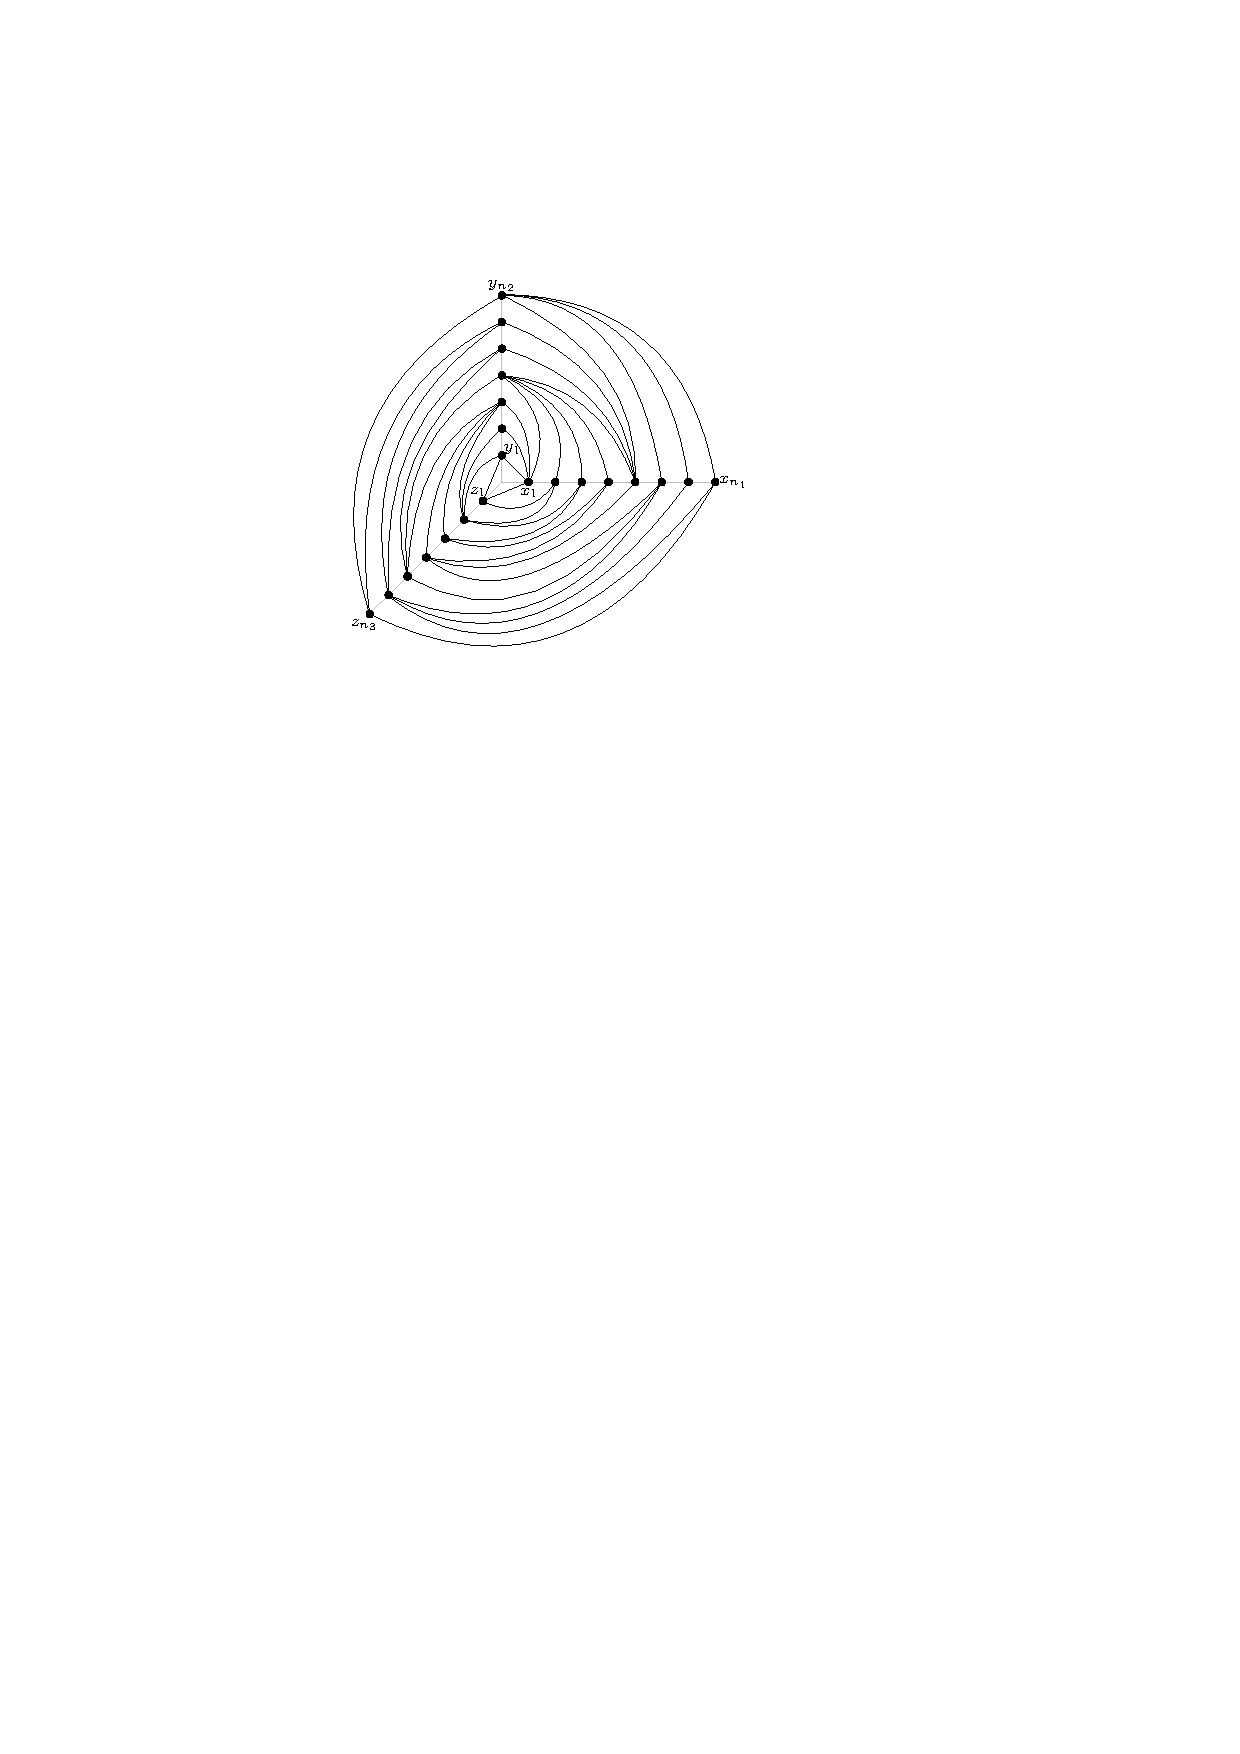
\includegraphics{figs/graph-1}
  \end{center}
  \caption{The standard planar embedding of a 3-track graph.}
  \figlabel{planar-view}
\end{figure}

Let $T_1,T_2,T_3$ be a 3-track layout of $G$ with
$T_1=\{x_1,\ldots,x_{n_1}\}$, $T_2=\{y_1,\ldots,y_{n_2}\}$, and
$T_3=\{z_1,\ldots,z_{n_3}\}$ and the total orders $\prec_1,\prec_2,\prec_3$
are implicit so that, for example $z_i\prec_3 z_j$ if and only if $i<j$.
In terms of \figref{planar-view}, this means that $x_1,y_1,z_1$ form
the triangular face containing the origin and $x_{n_1},y_{n_2},z_{n_3}$
form the cycle on the boundary of the outer face.
From this point onward, all track indices are implicitly taken ``modulo 3''
so that for any integer $i$, $T_i$ refers to the track $T_{i'}$ with
index $i'=((i-1)\bmod 3)+1$.

The following observation follows from the fact that $G$ is edge-maximal.
\begin{obs}\obslabel{silly}
  For any two vertices of $G$ on distinct tracks, say $x_i$ and $y_j$, at least
  one of the following conditions is satisfied (see \figref{3-cases}):
  \begin{enumerate}
    \item $x_{i}y_{j}\in E(G)$; or
    \item there exists $x_{i'}y_{j'} \in E(G)$ with $i'>i$ and $j'<j$; or
    \item there exists $x_{i}y_{j'}\in E(G)$ with $j'>j$.
  \end{enumerate}
\end{obs}

\begin{figure}
   \begin{center}
     \begin{tabular}{ccc}
       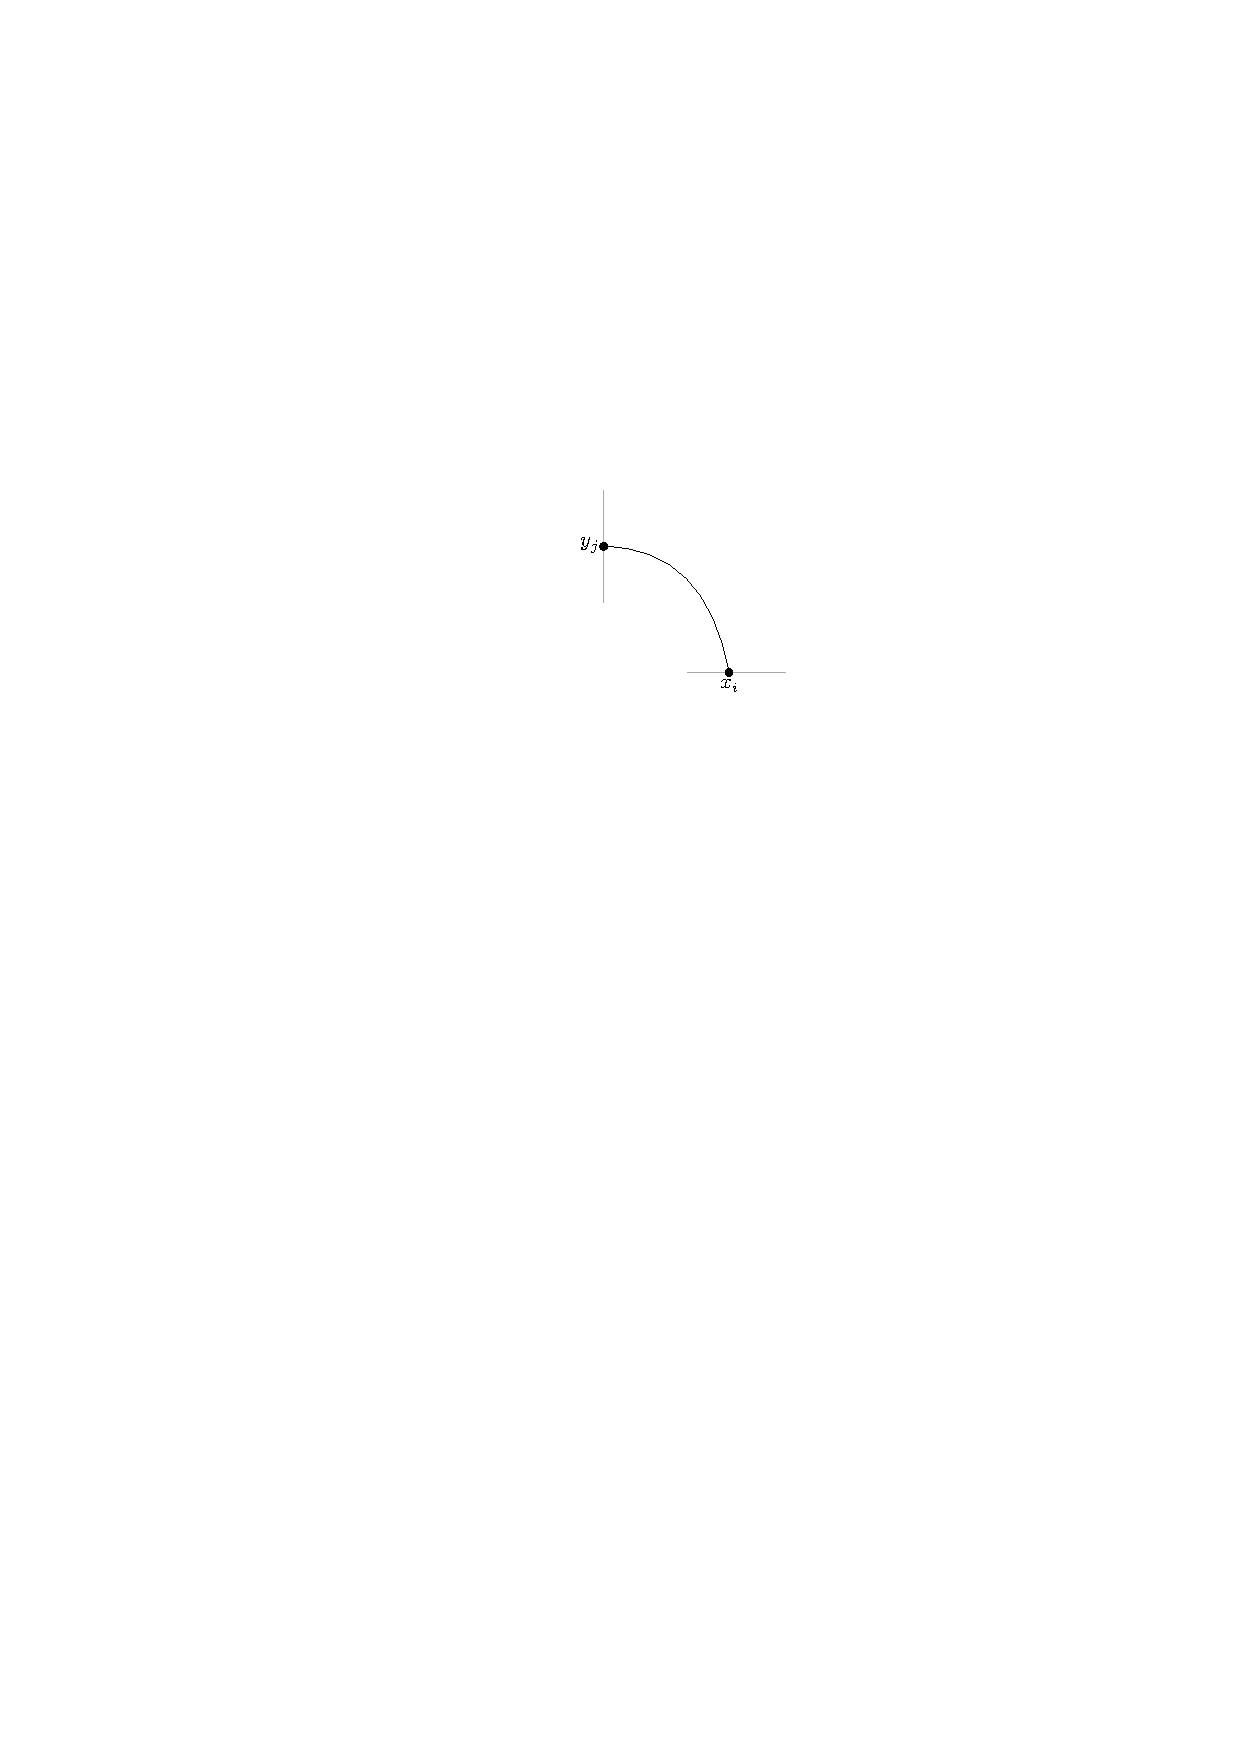
\includegraphics{figs/silly-1} &
       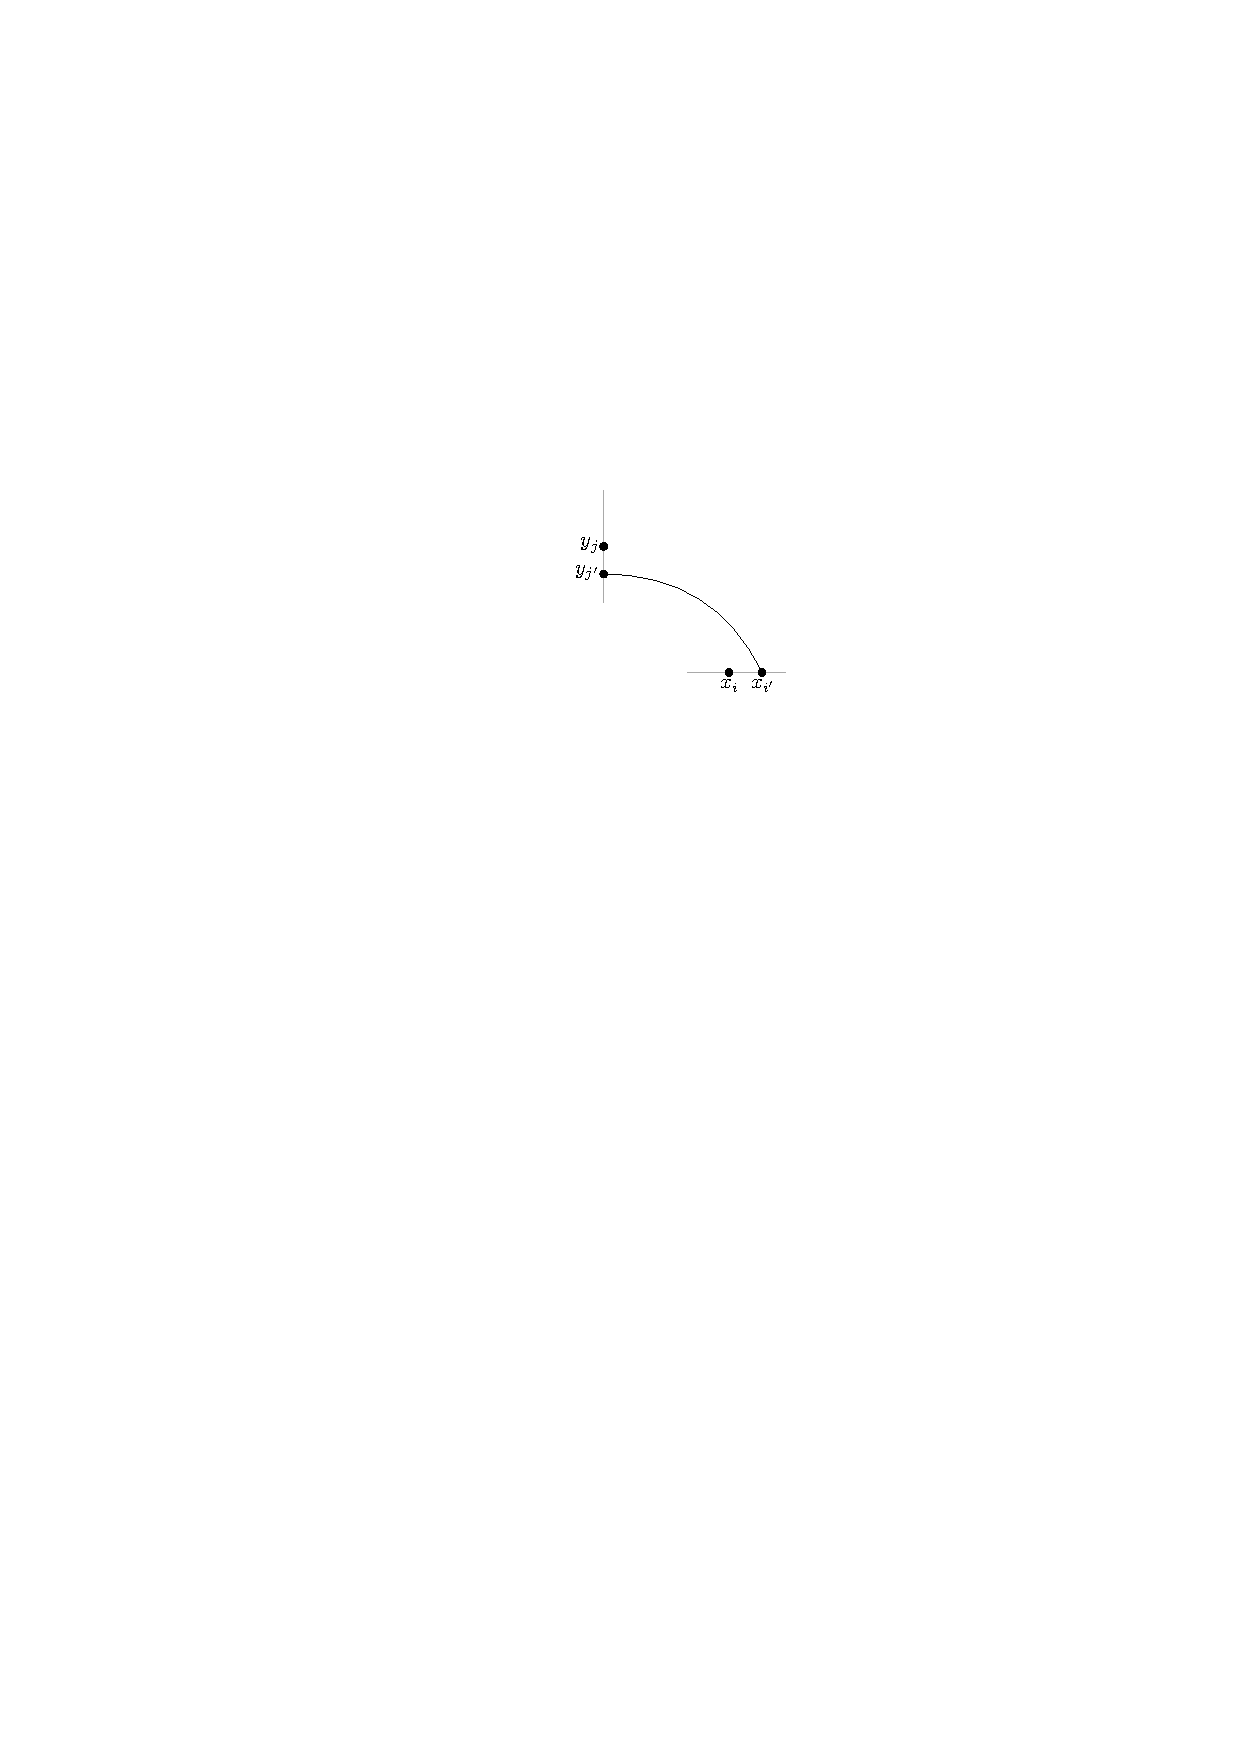
\includegraphics{figs/silly-2} &
       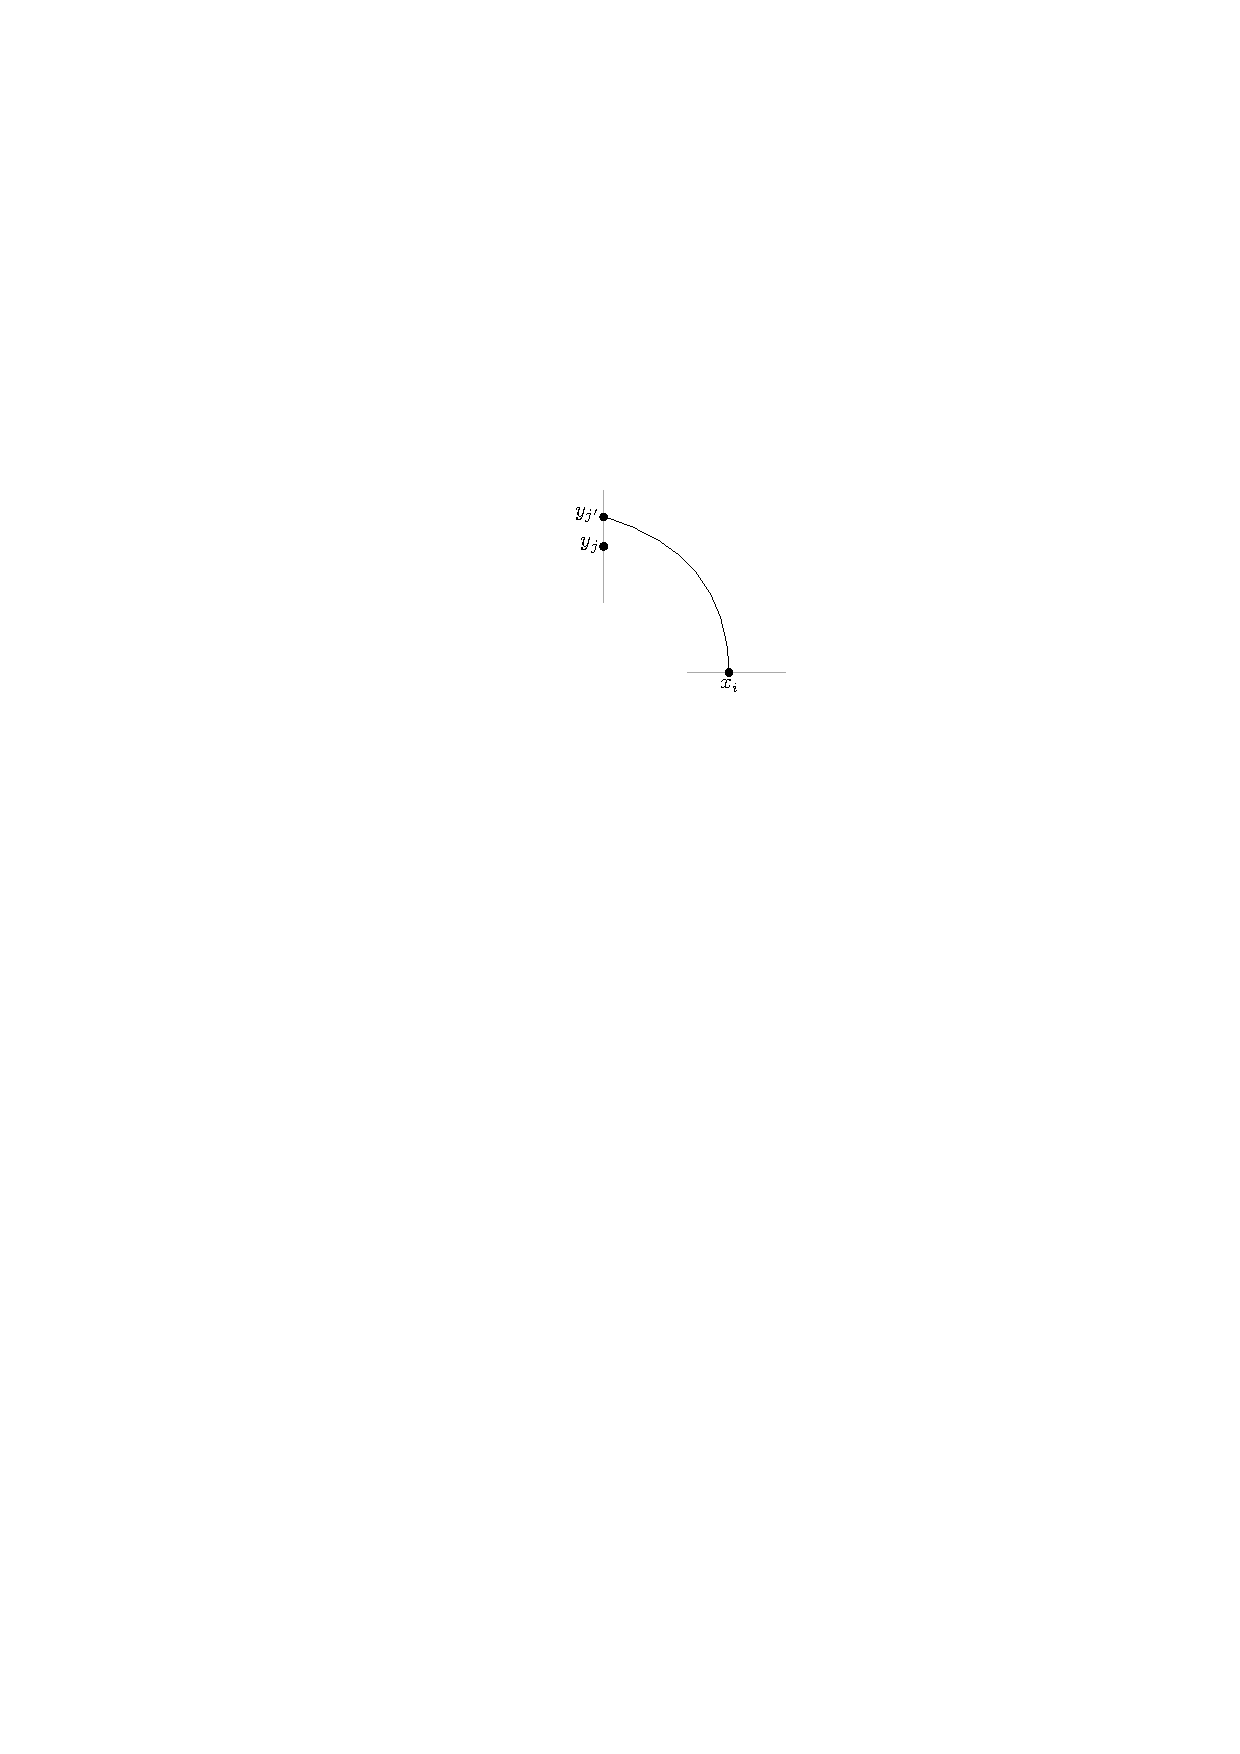
\includegraphics{figs/silly-3} \\
       (1) & (2) & (3)
     \end{tabular}
   \end{center}
   \caption{The three cases in \obsref{silly}.}
   \figlabel{3-cases}
\end{figure}


\thmref{main} is a consequence of the following lemma.

\begin{restatable}{lem}{main}\lemlabel{main}
  The edge-maximal 3-track graph $G$ with tracks $x_1,\ldots,x_{n_1}$, $y_1,\ldots,y_{n_2}$, and $z_1,\ldots,x_{n_3}$ described above has a 2-weak layered path
  decomposition, $B_1,\ldots,B_p$, with a layering $\ell$ of (layered) pathwidth $2$ in which
  \begin{enumerate}
    \item for each $i\in\{1,2,3\}$ and each $v\in T_i$,
      $\ell(v)\equiv i\pmod 3$;
    \item $B_1=\{x_1,y_1,z_1\}$;
    \item $\ell(x_1)=1$, $\ell(y_1)=2$, and $\ell(z_1)=3$;
    \item $B_p=\{x_{n_1},y_{n_2},z_{n_3}\}$; and
    \item $x_{n_1},y_{n_2},z_{n_3}$ appear in 3 distinct consecutive layers.
  \end{enumerate}
\end{restatable}

Before proving \lemref{main}, we show how it implies \thmref{main}.
Since layered pathwidth is monotone with respect to the addition of edges,
it is safe to assume (as \lemref{main} does) that $G$ is edge-maximal.
By \lemref{main}, therefore $G$ has $\lpw_2(G)\le2$ and therefore, by
\lemref{weak}, $\lpw(G)\le 4$.

\begin{proof}[Proof of \lemref{main}]
  The proof is by induction on the number of vertices of $G$.  If
  $|V(G)|\le 4$, then the result is trivial, so assume from this point onward that $|V(G)|\ge 5$.  Next, suppose that $G$ has
  a cut set $C=\{x_i,y_j,z_k\}$ having exactly one vertex in each track.
  Since $G$ is edge-maximal, $x_i,y_j,z_k$ form a cycle in $G$.  Now,
  the subgraph $G_1$ of $G$ induced by $\{x_1,\ldots,x_i, y_1,\ldots,y_j,
  z_1,\ldots,z_k\}$ is an edge-maximal graph with $\tr(G_1)=3$ and we
  can inductively apply \lemref{main} to find a width-2 2-weak layered
  path decomposition of $G_1$ in which $x_i,y_j,z_k$ are in the last bag
  and are assigned to three consecutive distinct layers $r+1$, $r+2$, and $r+3$.
  Note that there are three possible assignments of $x_i,y_j,z_k$ to
  these three layers depending on the value of $r\bmod 3$.  Suppose,
  without loss of generality, that $\ell(y_j)=r+1$ (so $\ell(z_k)=r+2$
  and $\ell(x_i)=r+3$.)

  Next, consider the graph $G_2$ induced by
  $\{x_i,\ldots,x_{n_1},y_j,\ldots,y_{n_2},z_k,\ldots,z_{n_3}\}$.
  We apply \lemref{main} inductively on $G_2$ relabelling tracks to
  ensure that in the resulting layered decomposition $\ell(y_j)=1$,
  $\ell(z_k)=2$ and $\ell(x_i)=3$.   We can now obtain a width-2 2-weak
  layered path decomposition of $G$ by joining the two decompositions.
  In particular, concatenating the sequence of bags for $G_1$ with
  the sequence of bags for $G_2$ gives a path decomposition of $G$
  and adding $r$ to the indices of all layers in the layering of $G_2$
  gives a 2-weak layering of $G$.

  Thus, all that remains is to study the case where $G$ contains no cut
  set having exactly one vertex on each track.  We claim that, in this
  case, $G$ contains the edge $x_1z_2$ or it contains the edge $z_1x_2$.
  Since $G$ is edge-maximal, this is obvious unless $n_1=n_3=1$ so
  that neither $z_2$ nor $x_2$ exist.  However, since $|V(G)|\ge 5$, $n_2\ge 3$, so  this would imply that $x_1,z_1,y_2$ is a cut set with one vertex on
  each track, since its removal separates all $y_1$ from $y_3$.

  We will construct a path $P=v_1,\ldots,v_r$, an example of which is illustrated in \figref{path}. The first vertex of $P$ will be one of
  $x_1,y_1,z_1$ and the final three vertices are $x_{n_1}$,
  $y_{n_2}$, and $z_{n_3}$, though not necessarily in that order.
  The path $P$ will \emph{spiral} in the sense that $v_i\in T_i$
  for all $i\in\{1,\ldots,r\}$.  Observe that this spiralling implies that the subsequence of vertices of $P$ on any track $T_i$ is increasing (getting further from the origin).

  \begin{figure}
     \begin{center}
        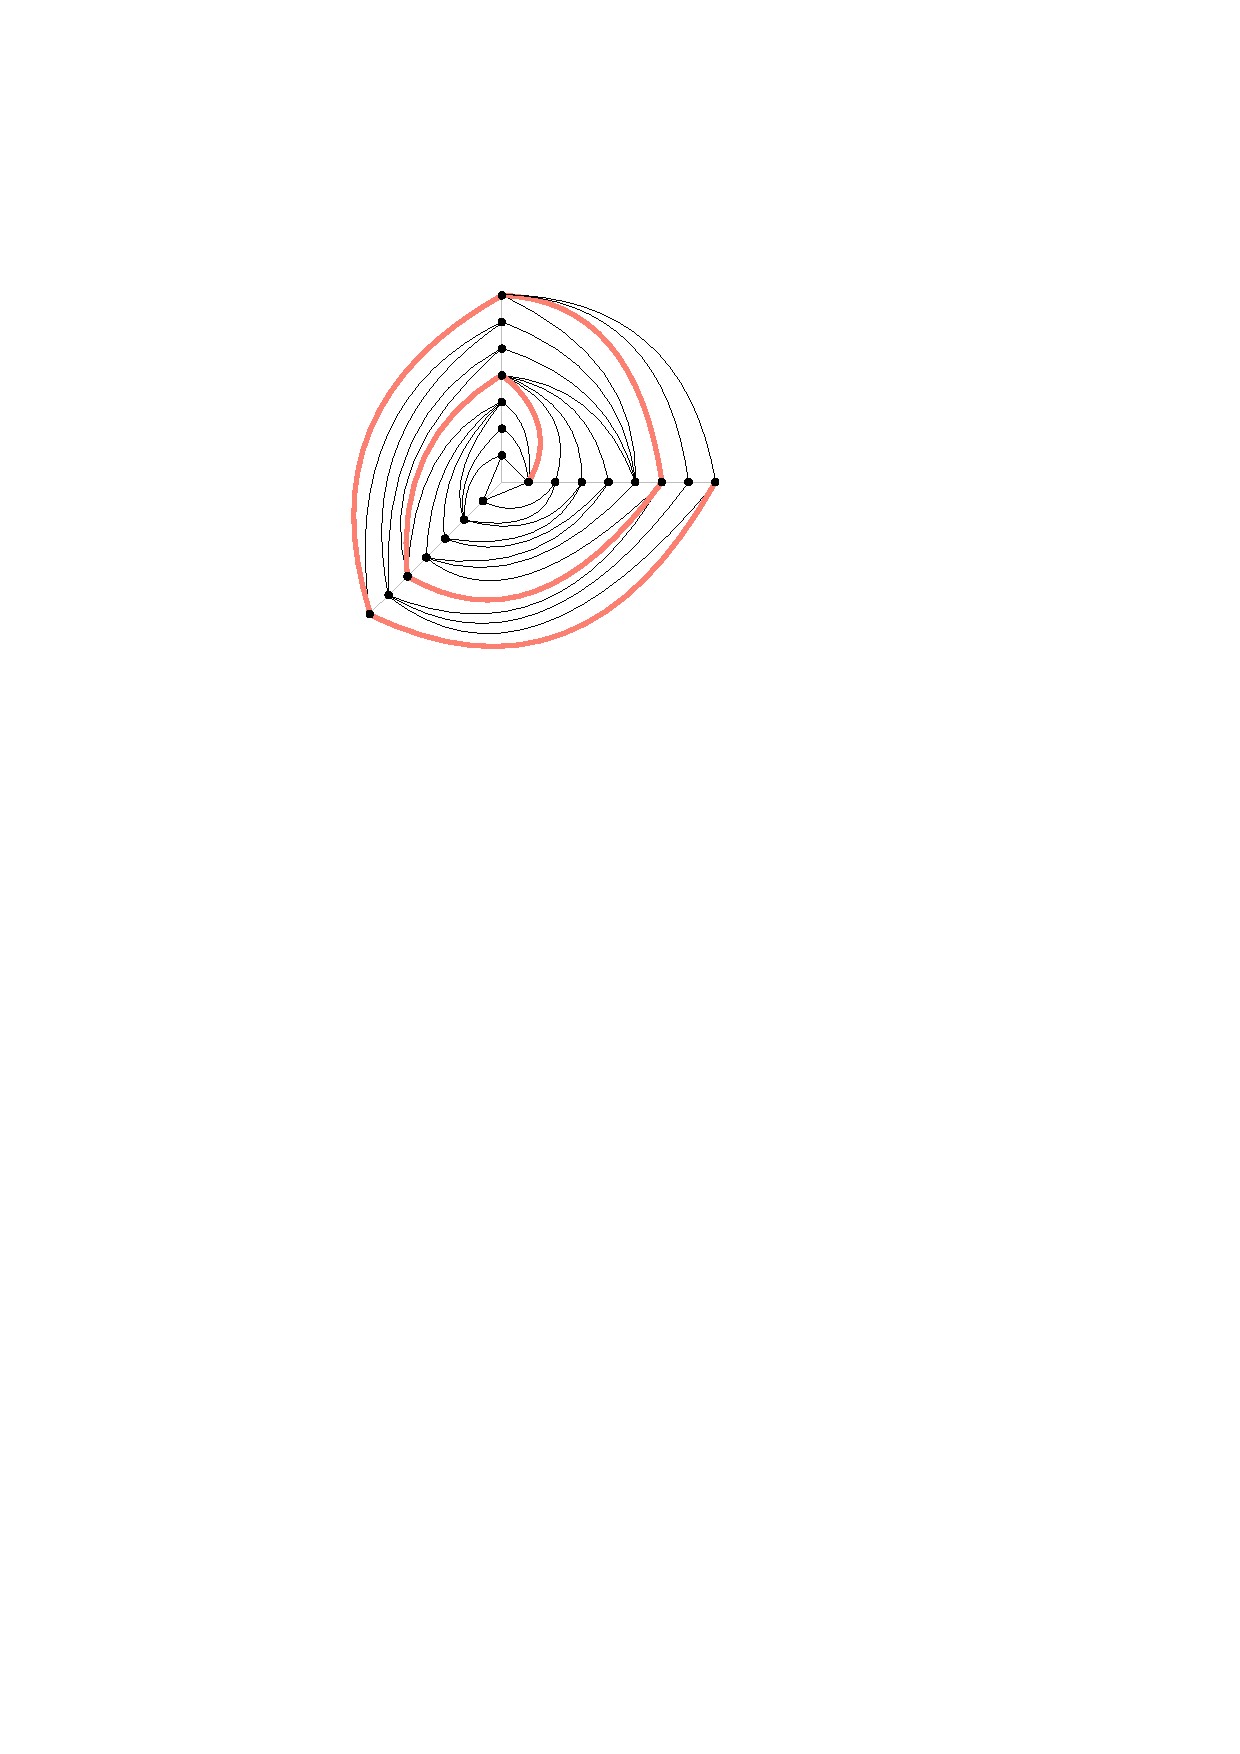
\includegraphics{figs/graph-2}
     \end{center}
     \caption{The path $P$ used in the proof of \lemref{main}.}
     \figlabel{path}
  \end{figure}

  $P$ is constructed greedily: if $P$ has reached vertex $v_k$, it continues to the neighbouring vertex
  $v_{k+1}$ of $v_{k}$ with the highest index on track $T_{k+1}$ that is not yet in $P$.
  We will call this vertex $v_{k+1}$ the \emph{furthest neighbouring vertex} of $v_k$.  To see why this is always possible,
  recall that $P$ already contains an edge $v_{k-3},v_{k-2}$. Now, without loss of generality we can
  apply \obsref{silly} with $x_i=v_k$ and $y_j=v_{k-2}$, so there
  are three cases (see \figref{sloppy}):

\begin{figure}
   \begin{center}
     \begin{tabular}{ccc}
       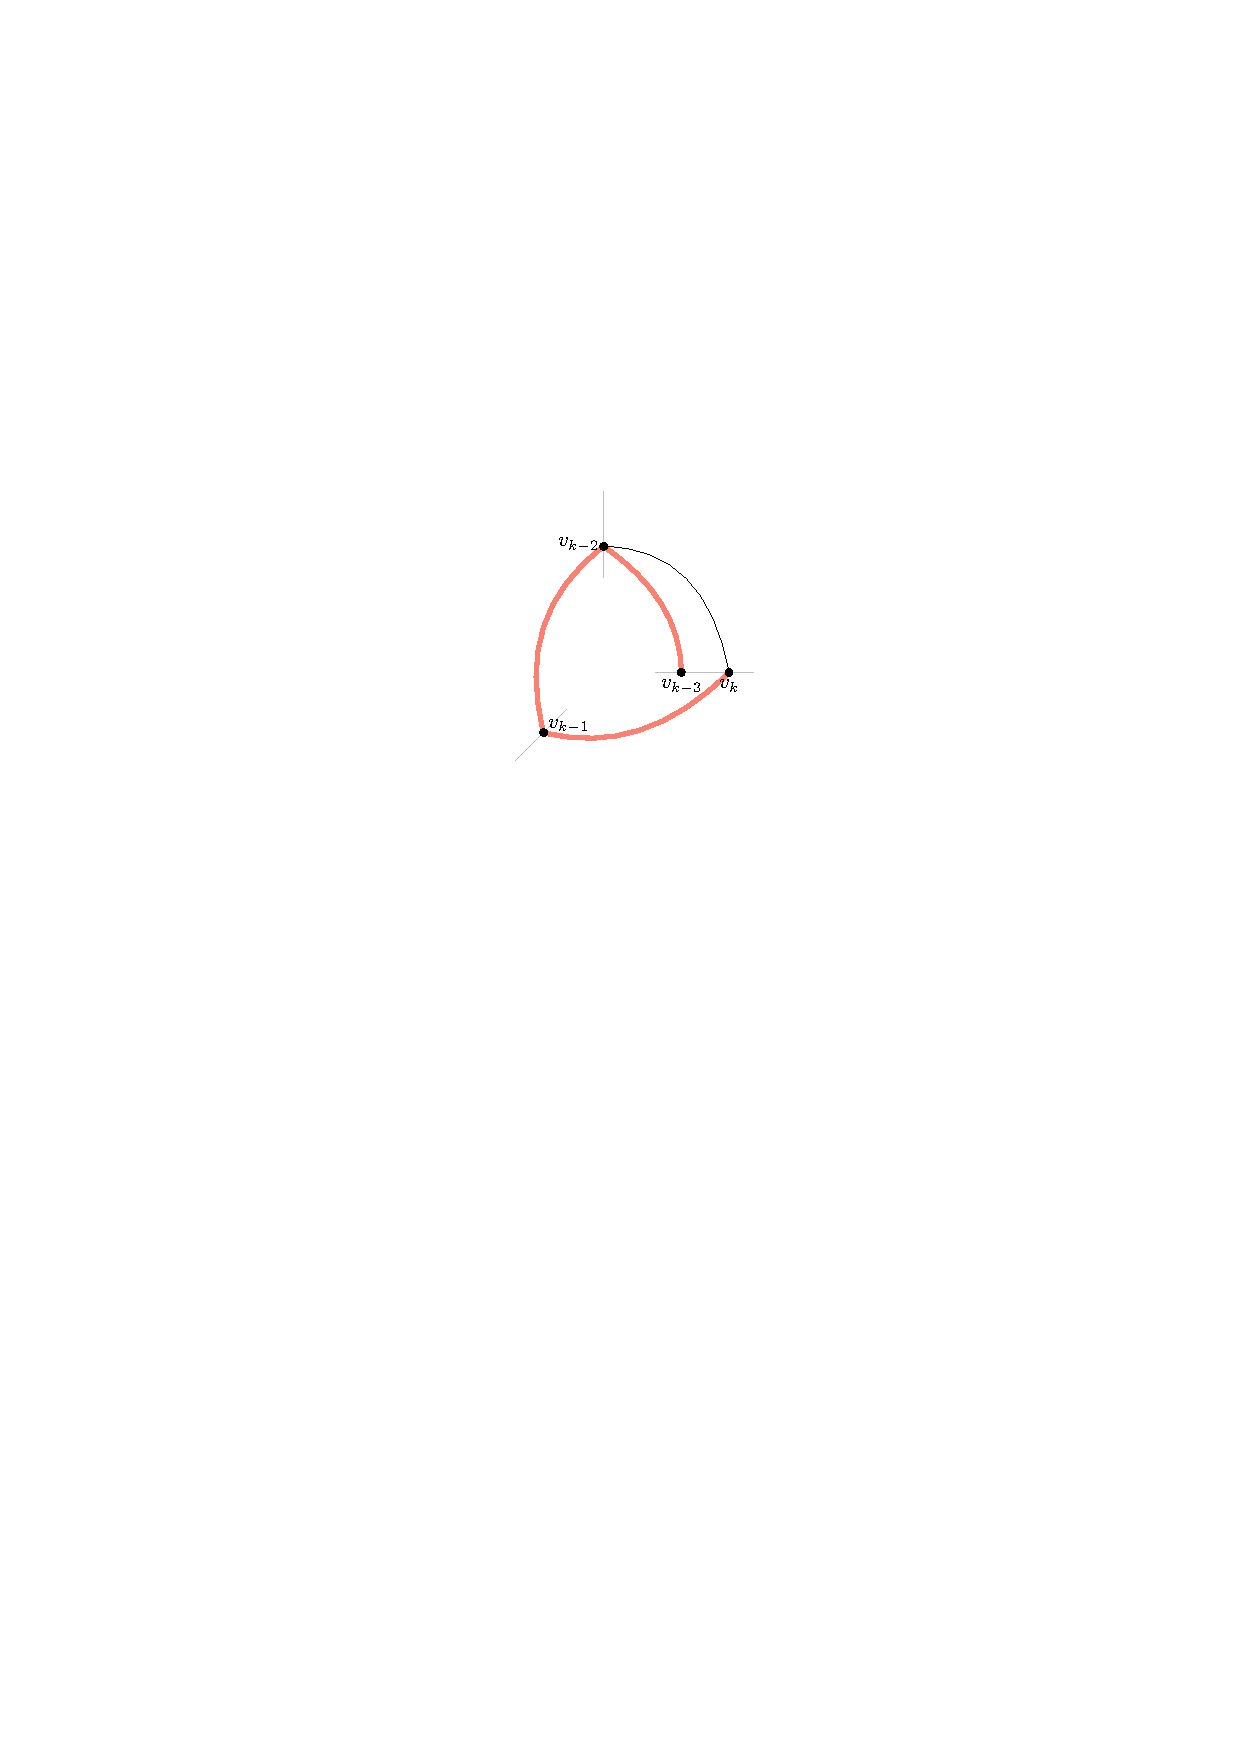
\includegraphics[width=0.3\columnwidth]{figs/sloppy-1} &
       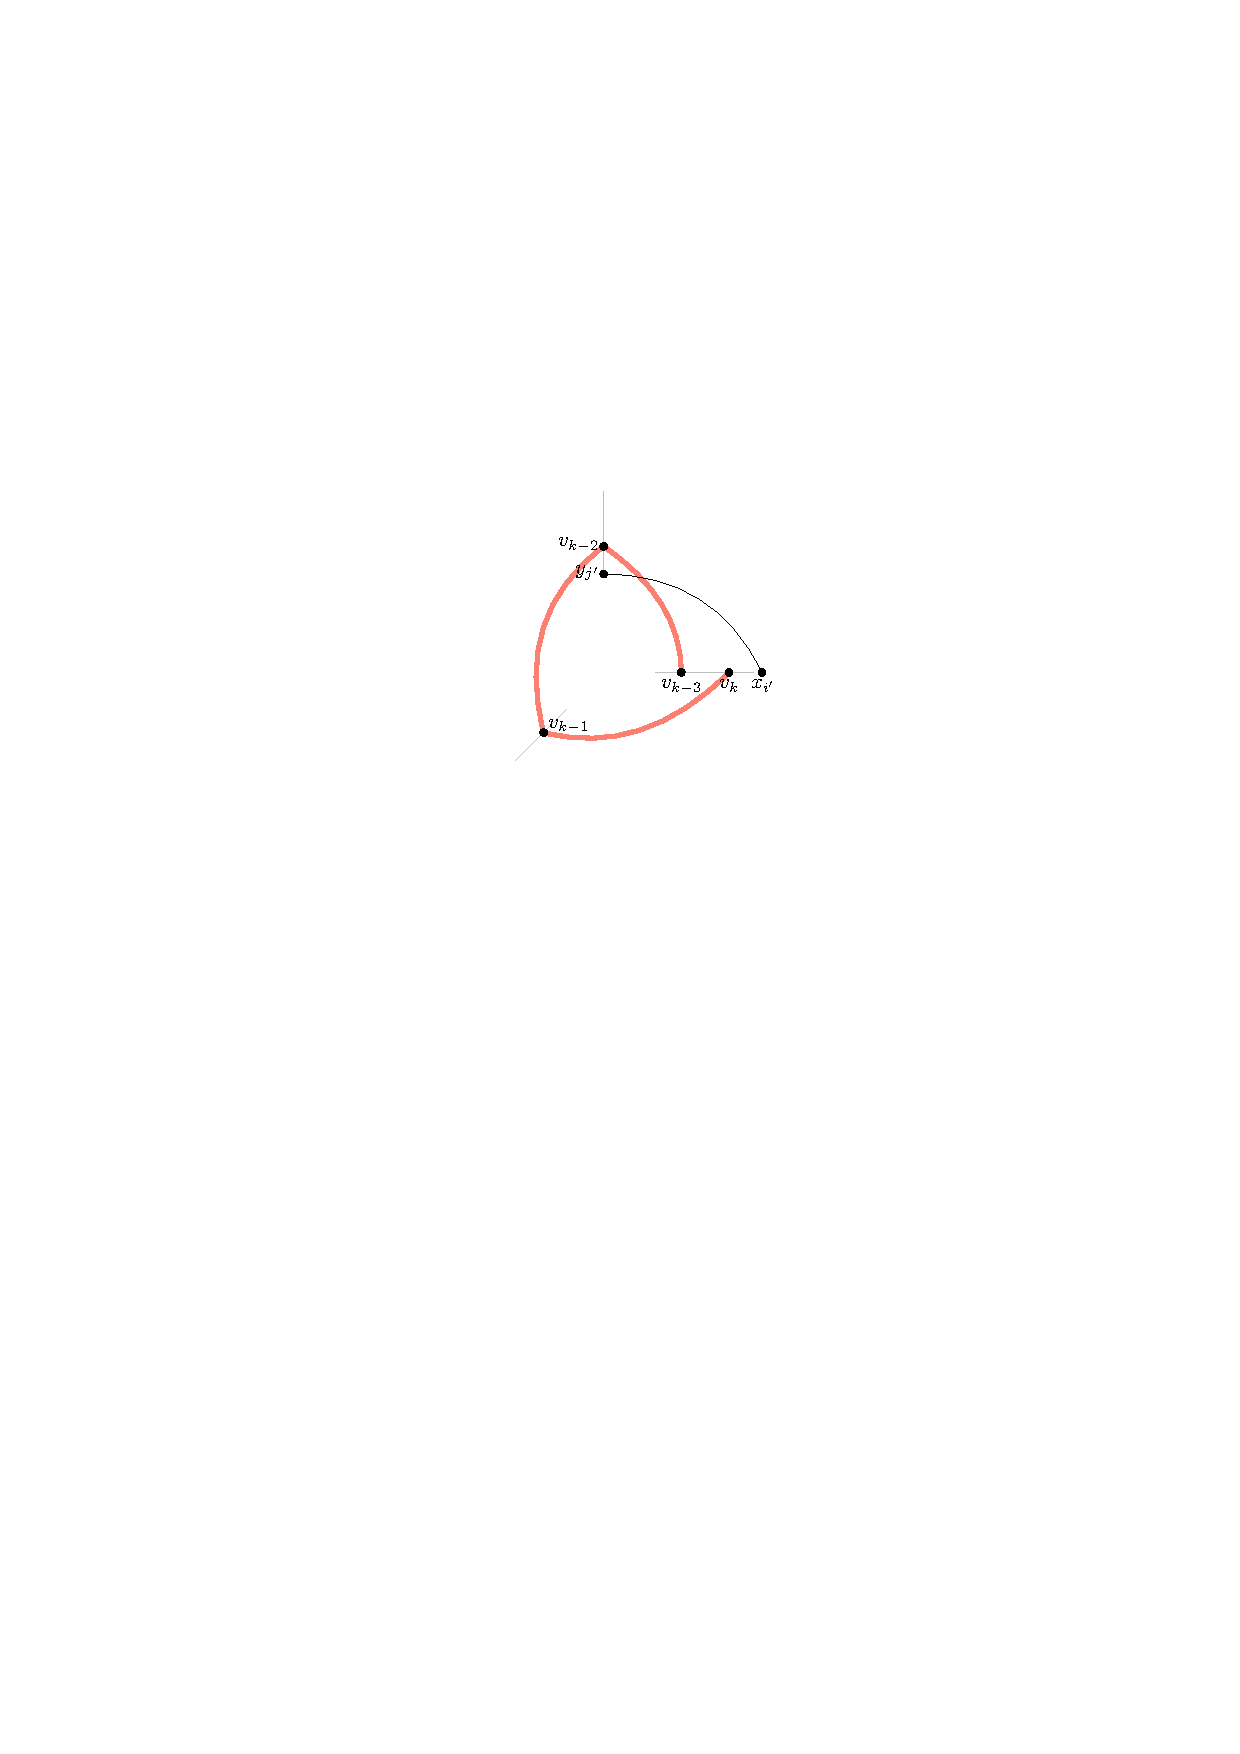
\includegraphics[width=0.3\columnwidth]{figs/sloppy-2} &
       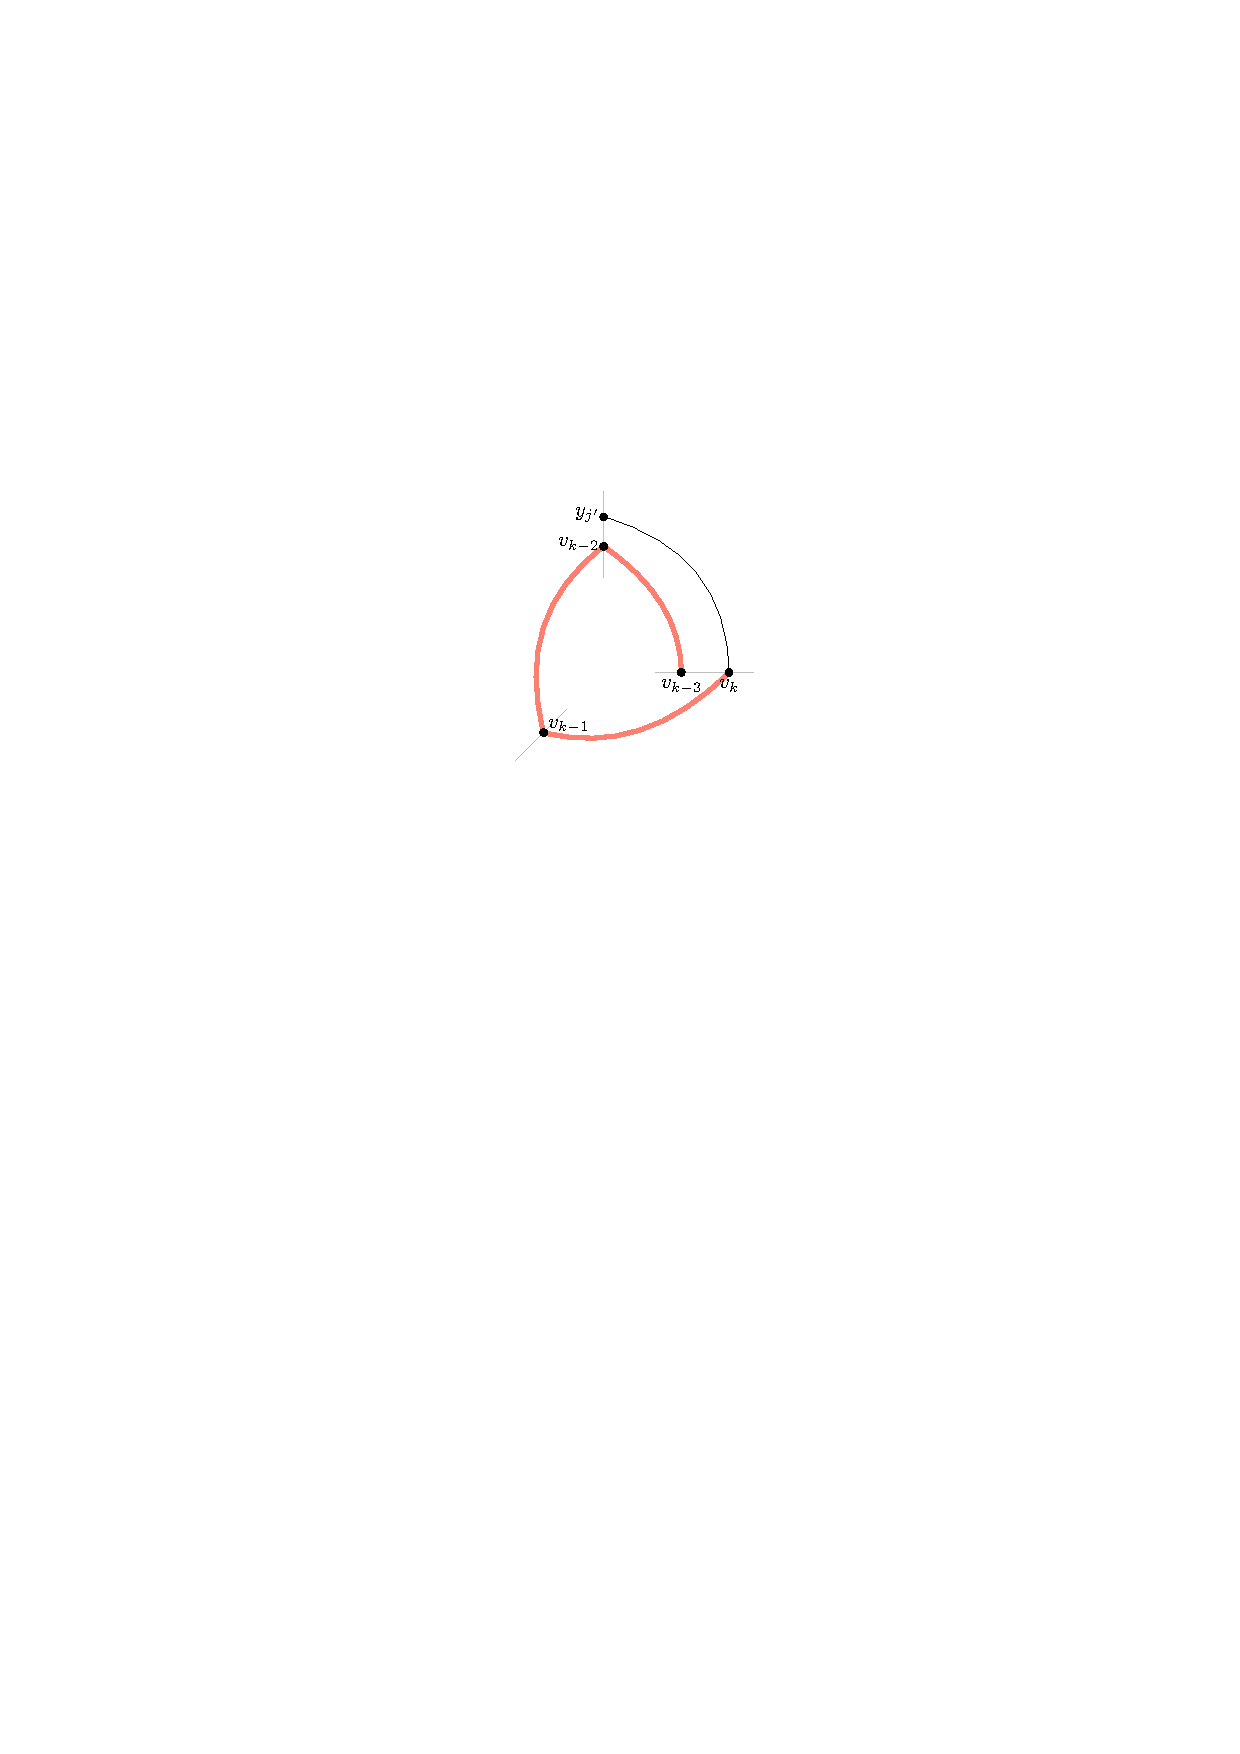
\includegraphics[width=0.3\columnwidth]{figs/sloppy-3} \\
       (1) & (2) & (3)
     \end{tabular}
   \end{center}
   \caption{The path $P$ can always be extended.}
   \figlabel{sloppy}
\end{figure}


  \begin{enumerate}
  \item $v_k v_{k-2}\in E(G)$.  In this
  case $v_{k-2}$, $v_{k-1}$, and $v_k$ form a cycle in $G$.  Then either
  $\{v_{k-2},v_{k-1},v_{k}\}=\{x_{n_1},y_{n_2},z_{n_3}\}$ or
  $\{v_{k-2},v_{k-1},v_{k}\}$ is a cut set with exactly one vertex in
  each track.  In the former case, the path $P$ is complete. The latter case is  excluded by the assumption that $G$ contains no such cut sets.

  \item there exists an edge $x_{i'}y_{j'}\in E(G)$ with $i' > i$
    (i.e. $i' > k$) and $j'< j$ (i.e. $j'< k-2$).  This case is not possible, since this edge would cross $v_{k-3}v_{k-2}$.

  \item there exists an edge $v_k y_{j'}\in E(G)$ with $j' >j$  (i.e. $j'> k-2$).  In this case, $P$ is extended by adding $v_{k+1}=y_{j'}$.
  \end{enumerate}


  Thus we have constructed the furthest vertex path $P=v_1,\ldots,v_r$ whose first vertex is one of
  $x_1,y_1,z_1$ and whose last three vertices are $x_{n_1}$,
  $y_{n_2}$ and $z_{n_3}$ (not necessarily in order).  We assign layers
  to the vertices of $P$ as follows: For each vertex $v_i$ on $P$,
  we set $\ell(v_i)=i$.  Note that this satisfies Conditions~3 and 5
  of the lemma and also satisfies Condition~1 for the vertices of $P$.
  For each $t\in\{1,2,3\}$, any vertex $v\in T_t$ that is not in
  $P$ is assigned to the same layer as $v$'s immediate successor in $P\cap T_t$.
  This assignment satisfies Condition~1 for vertices not in $P$.
  Finally, we will prove that this gives a 2-weak layering of $G$. In other words,
  in the worst case, a vertex $v$ with $\ell(v)=i$ can only share an edge with vertex $u$ where  $i-2 \le \ell(u) \le i+2$.

 Any edge between $v$ and $w$ where neither $v$ nor $w$ is in $P$ will only span one layer.
 Any edge between any two vertices $v_i$ and $v_j$ where $v_i, v_j \in P$, will span only one layer if $j = i\pm1$.
 This would mean that $v_{i}v_{j}$ is an edge in the graph $G$
 and that this edge was used to construct our furthest vertex path $P$.
 If $j \neq i\pm1$, then there are two cases:
   \begin{enumerate}
	\item $j = i \pm 2$ Such an edge is possible, and allowed since it spans only two layers. % and would create a cut set. This edges will only span 2 layers since $\ell(v_i) = i$ and $\ell(v_j) = i+2$.
	\item $j = i \pm 4$ Such an edge cannot exist since it would contradict our greedy path constructing algorithm.
	If the edge $v_iv_{i+4}$ (or the edge $v_{i-4}v_i$) existed then the edge $v_i v_{i+1}$ ($v_{i-4}v_{i-3}$ ) would not have been added to $P$.
   \end{enumerate}

 Any edge between $v$ and $w$ where $v \in P$ and $w \not\in P$ will be one of 7 types (see \figref{2layermaximum}).
 Without loss of generality, assume the spiral is travelling from $T_1$ to $T_2$ to $T_3$. Let $x_i$ be a vertex on the constructed path $P$.
 First, we look at the possible cases for an edge between $x_i$ with $\ell(x_i) = m$ and $y_j$ where $y_j \notin P$.


 \renewcommand{\thesubfigure}{\arabic{subfigure}}
  \begin{figure}
    \begin{center}
    \begin{subfigure}[t]{0.3\hsize}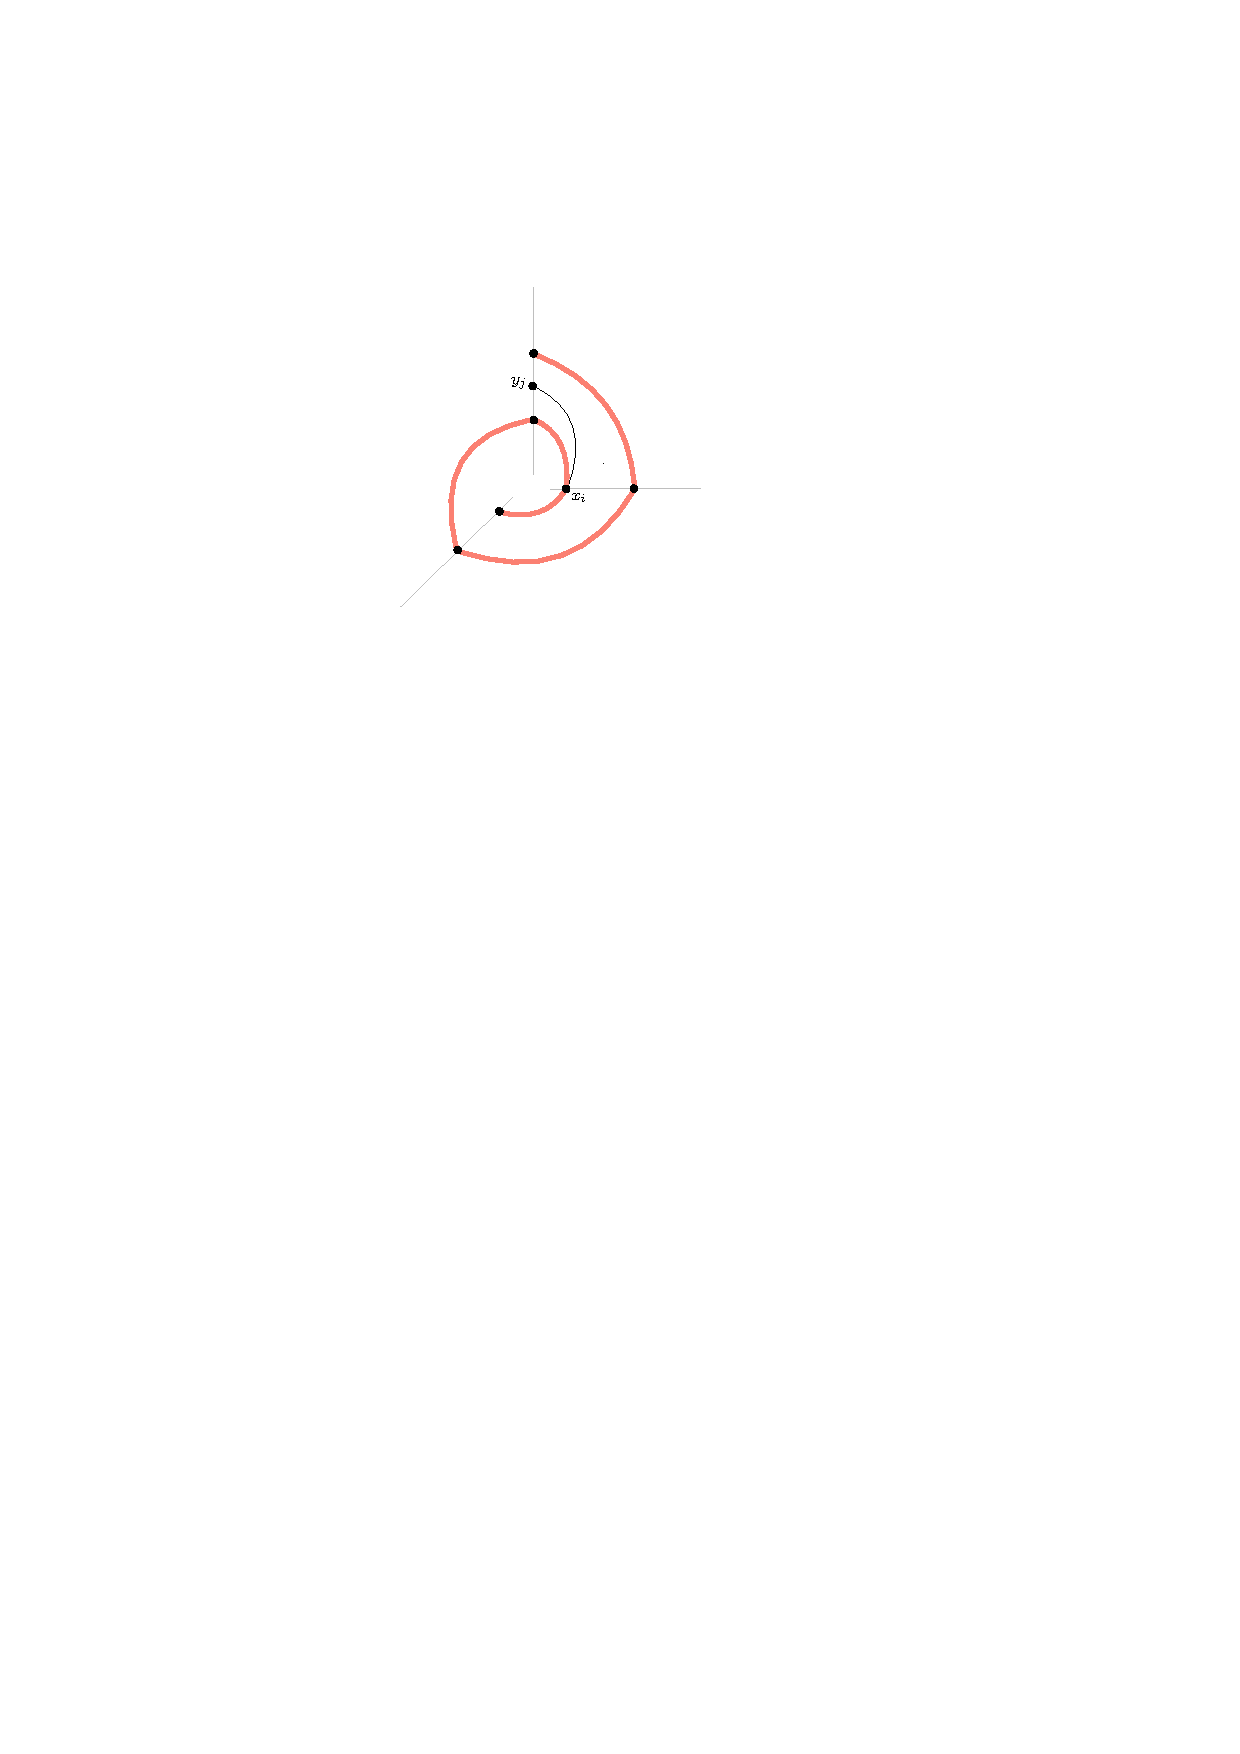
\includegraphics[width=40mm]{figs/2layermaximum-1} \caption{}\end{subfigure}
    \begin{subfigure}[t]{0.3\hsize}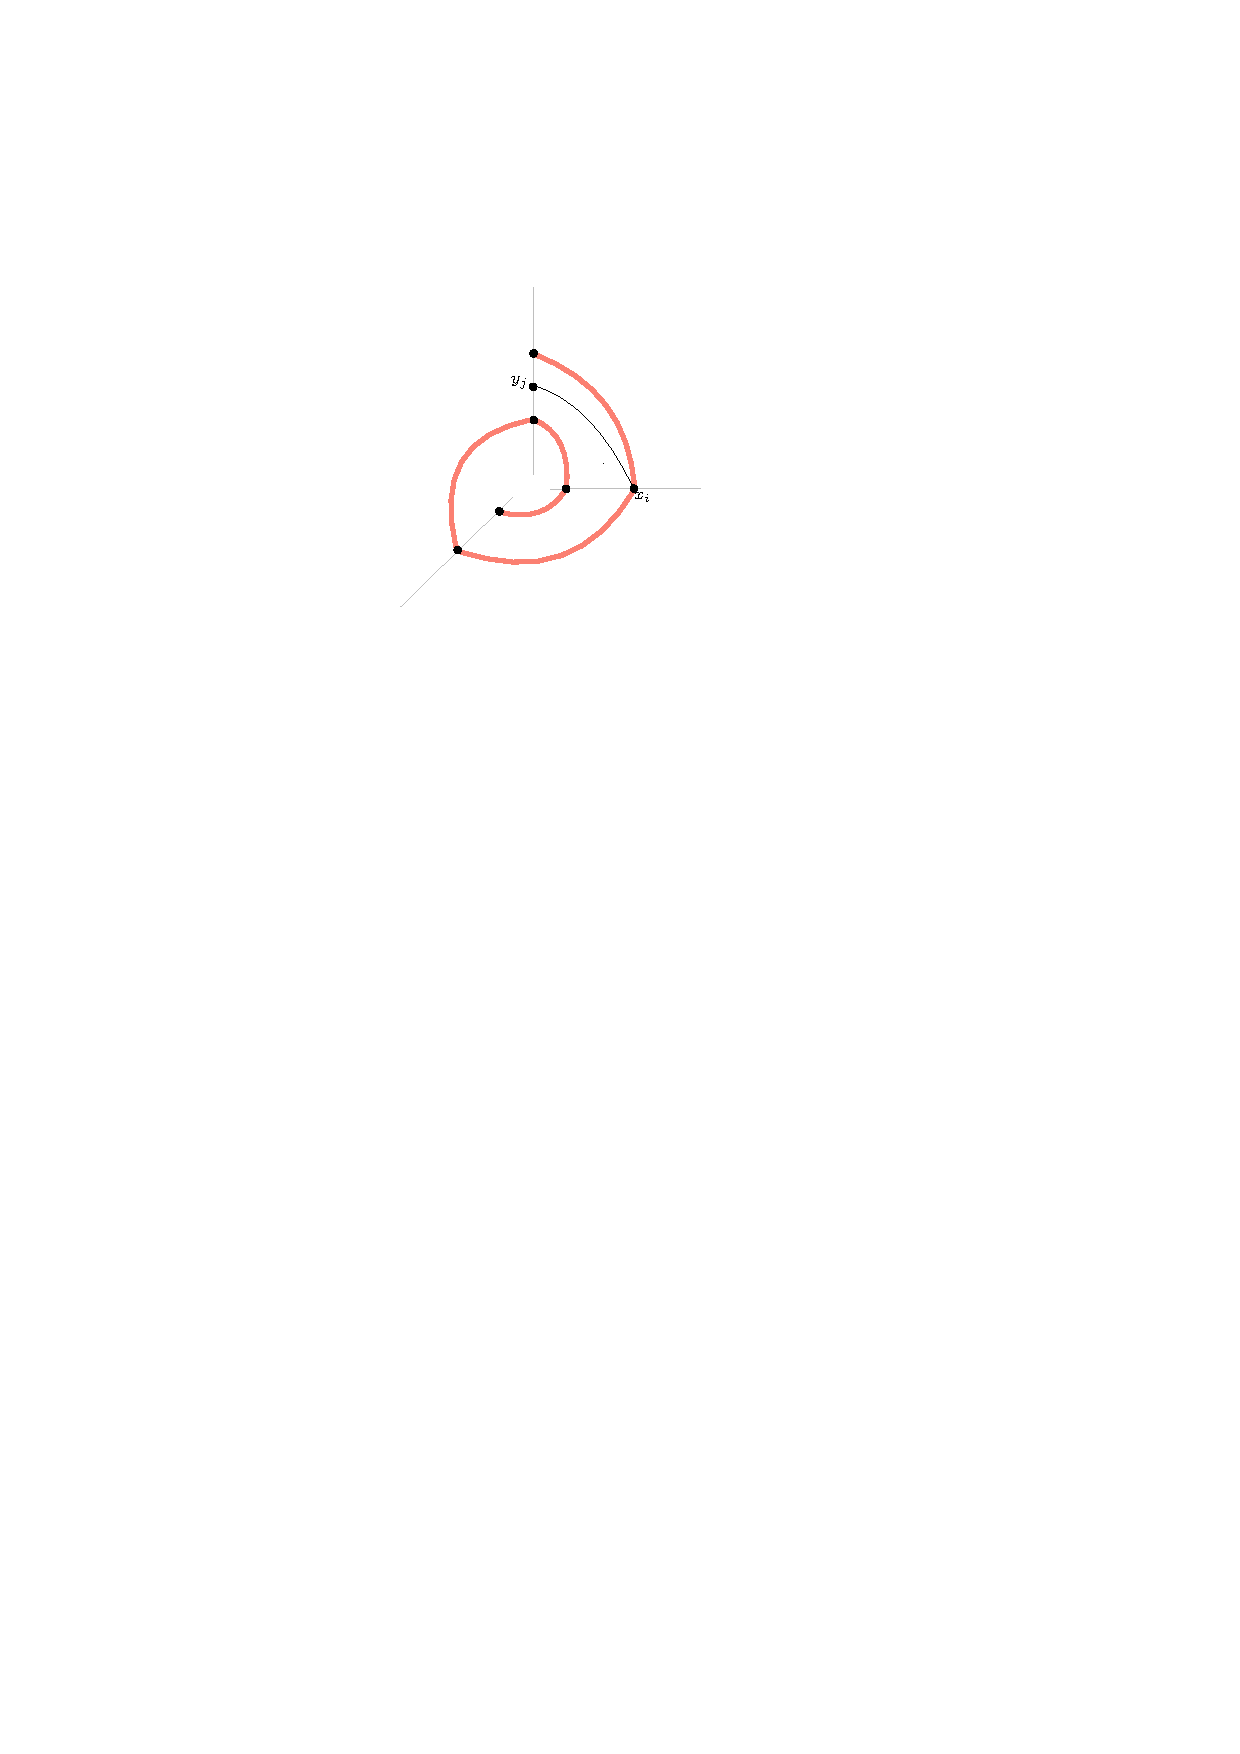
\includegraphics[width=40mm]{figs/2layermaximum-2} \caption{}\end{subfigure}
    \begin{subfigure}[t]{0.3\hsize}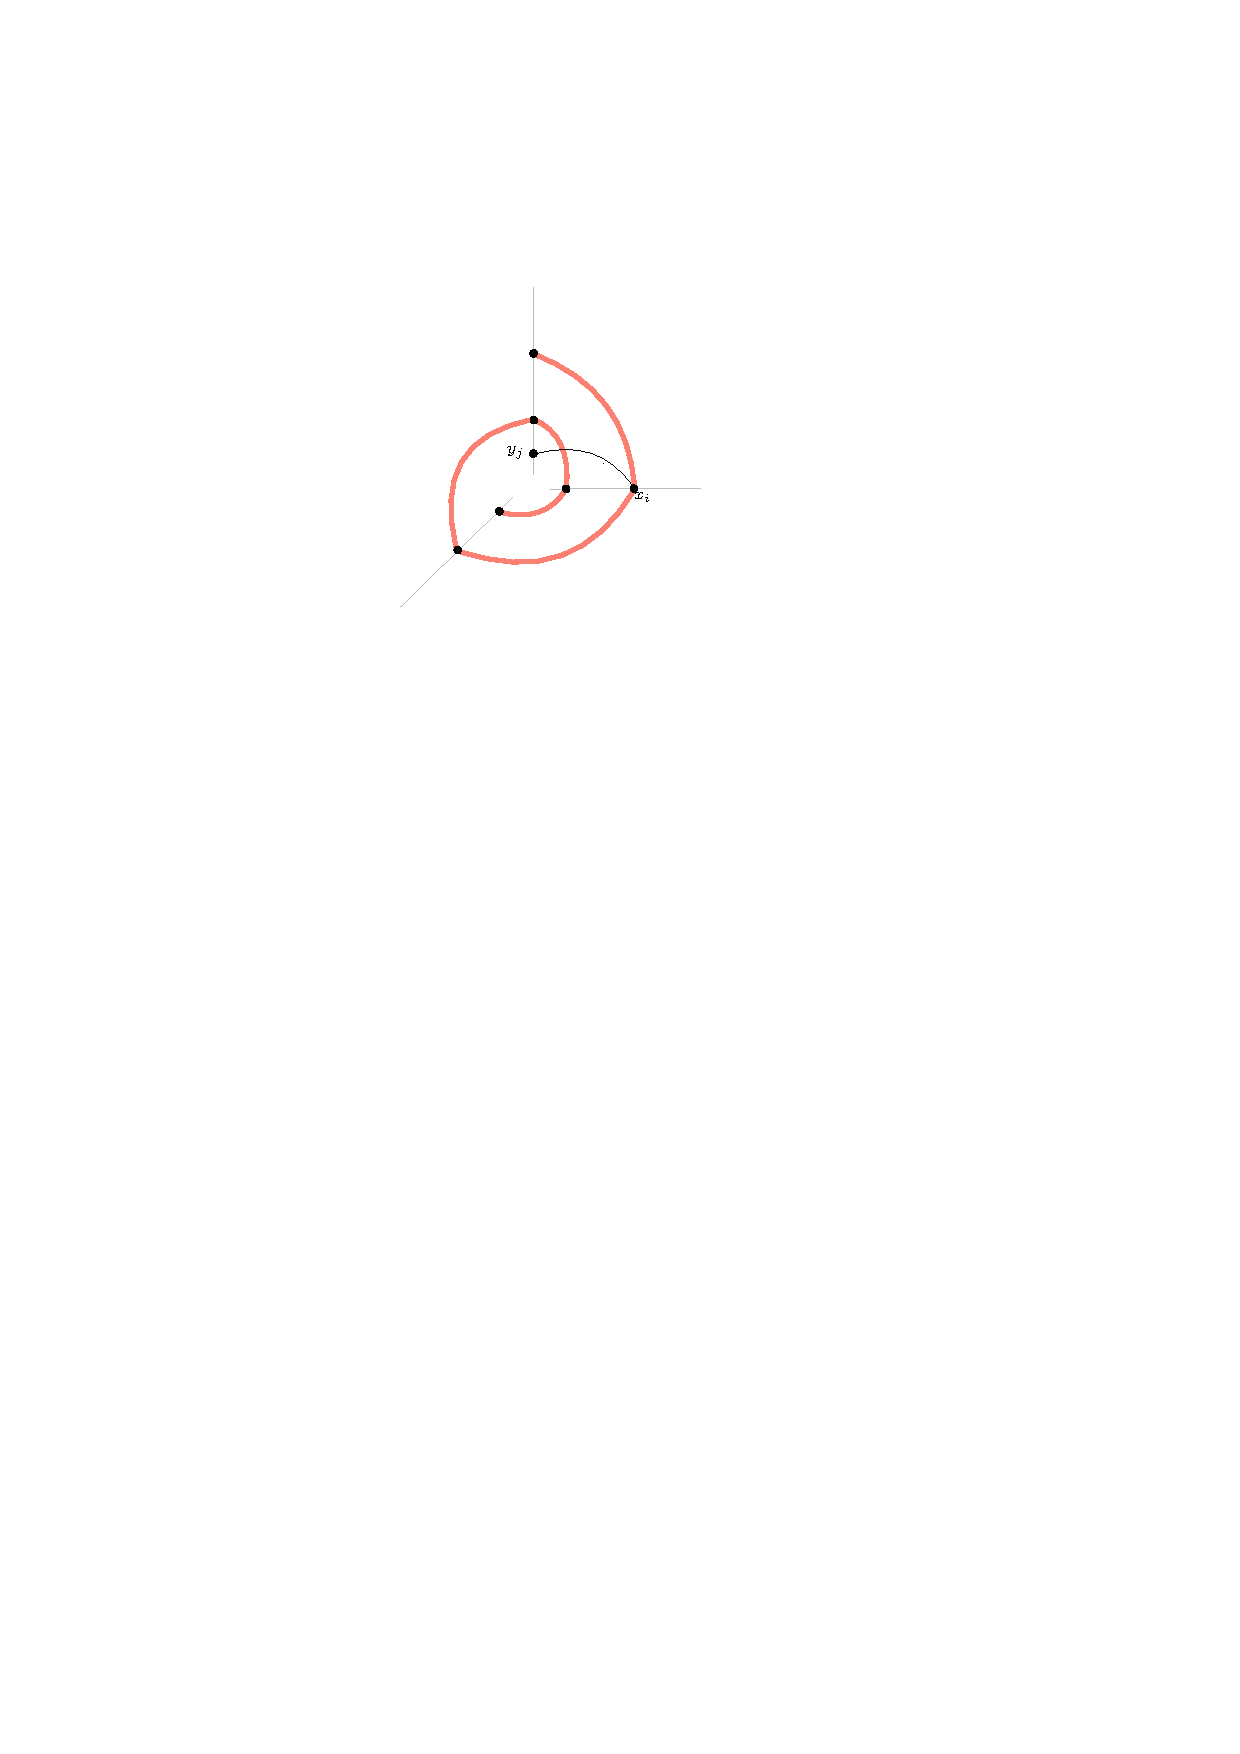
\includegraphics[width=40mm]{figs/2layermaximum-3} \caption{}\end{subfigure}
    \\[2ex]
    \begin{subfigure}[t]{0.4\hsize}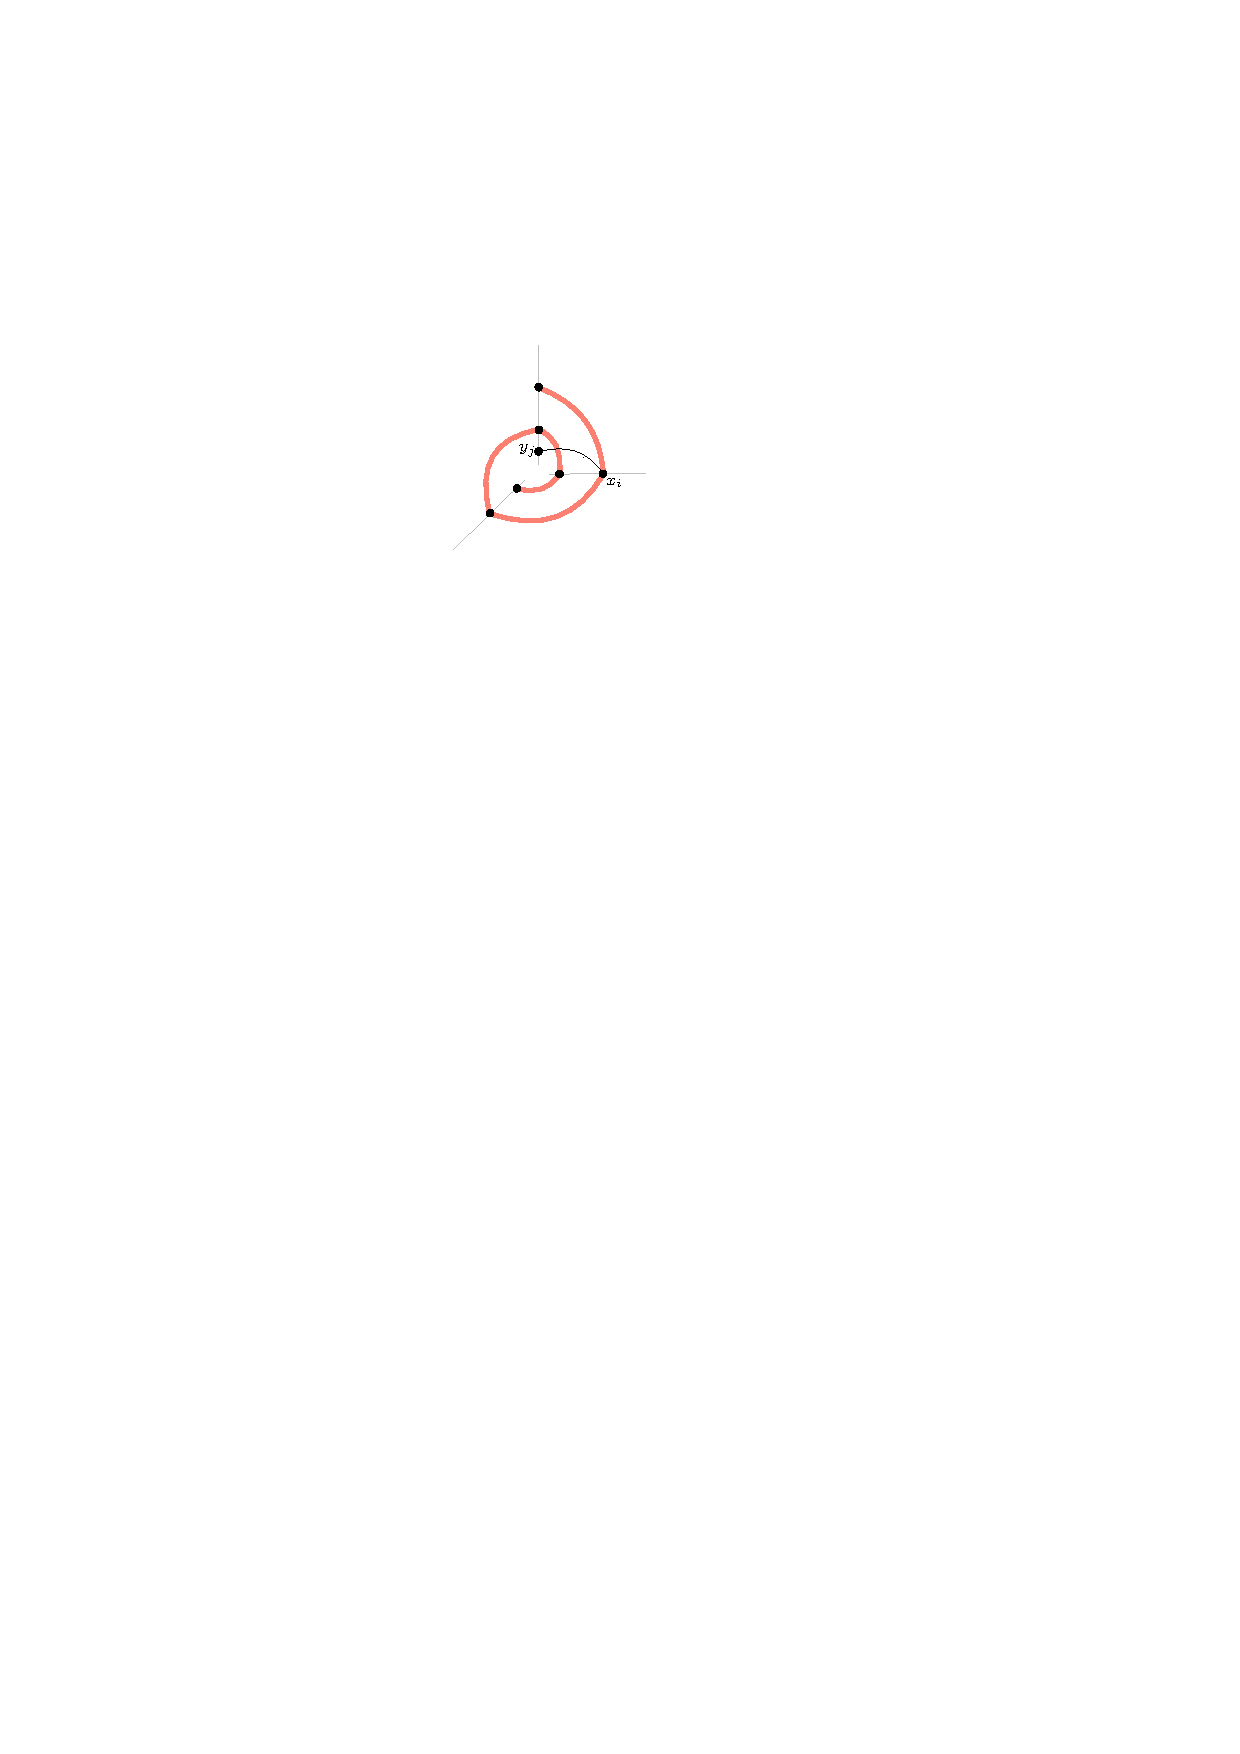
\includegraphics[width=40mm]{figs/2layermaximum-4} \caption{}\end{subfigure}
    \begin{subfigure}[t]{0.4\hsize}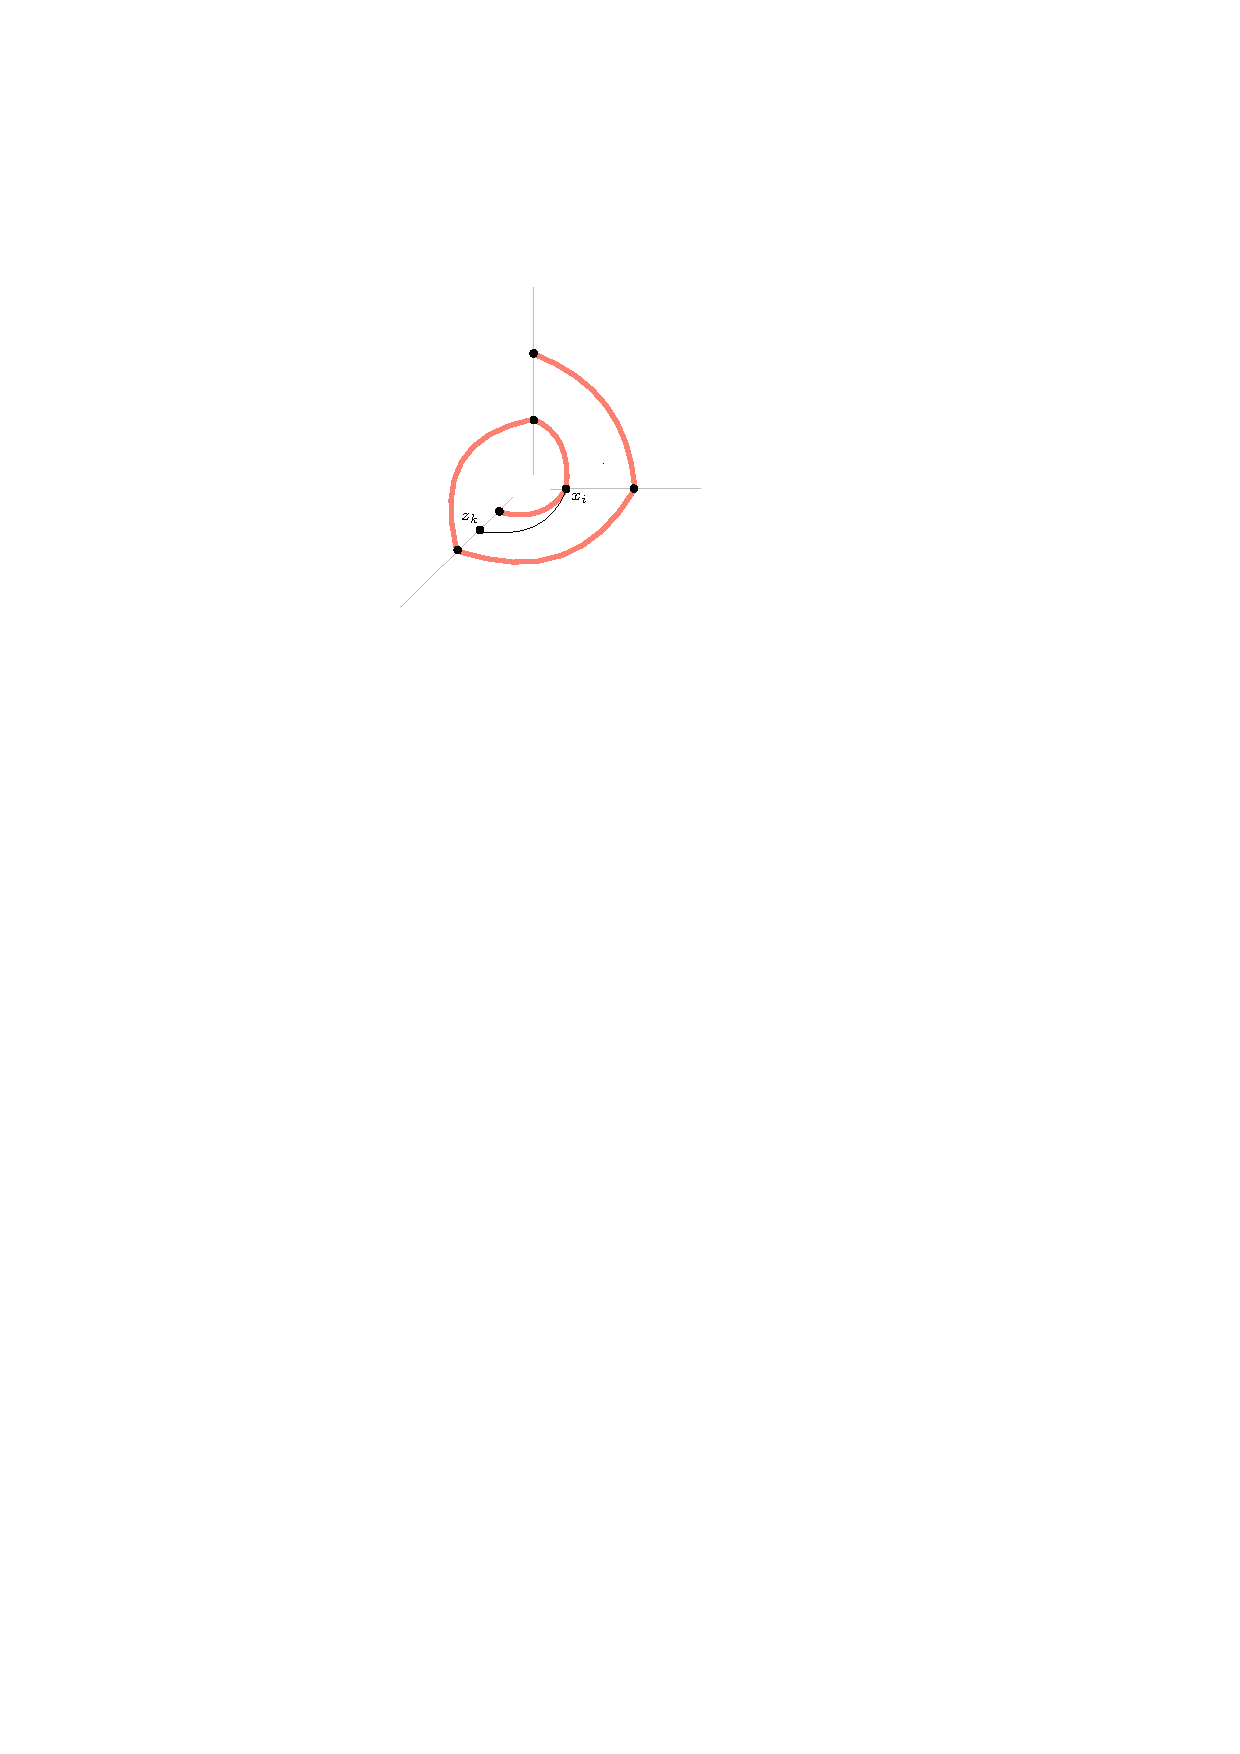
\includegraphics[width=40mm]{figs/2layermaximum-5} \caption{}\end{subfigure}
    \\[2ex]
    \begin{subfigure}[t]{0.4\hsize}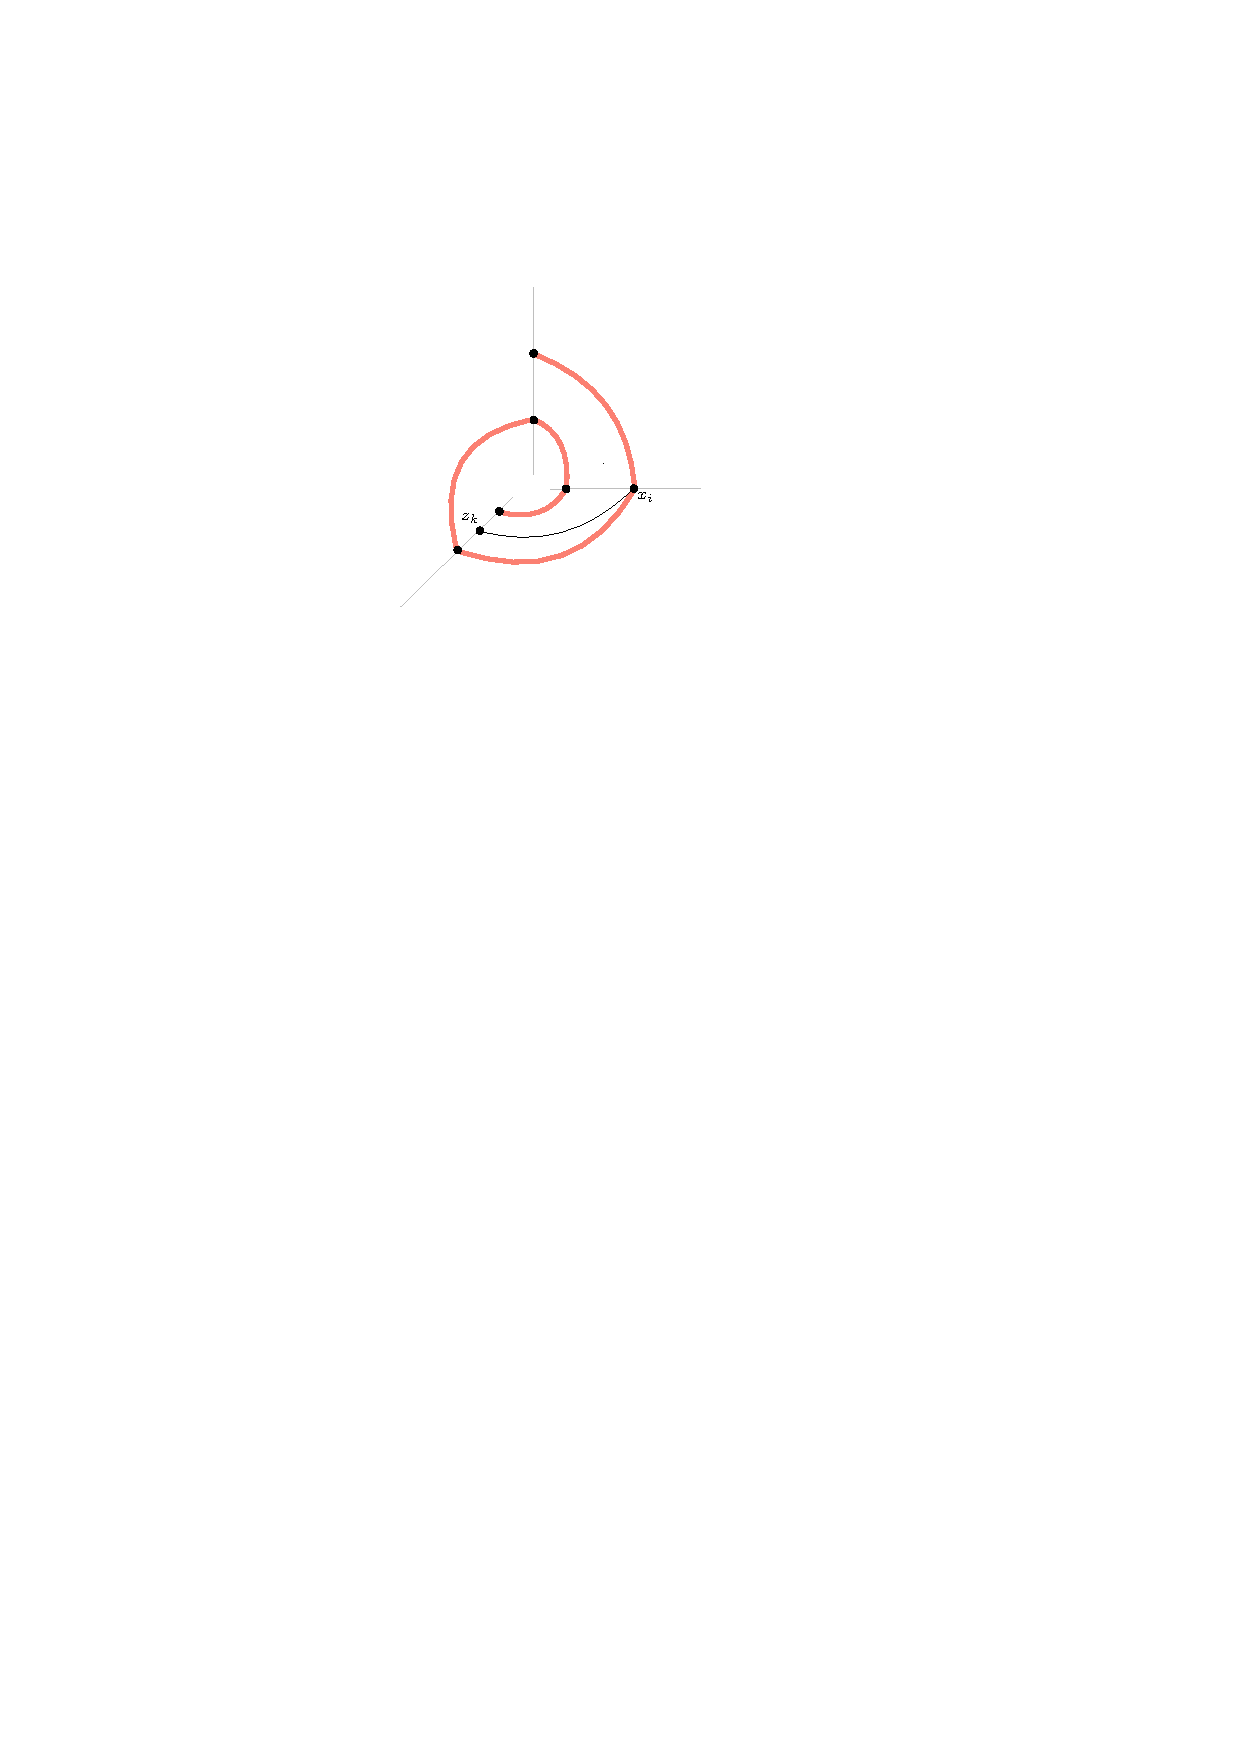
\includegraphics[width=40mm]{figs/2layermaximum-6} \caption{}\end{subfigure}
    \begin{subfigure}[t]{0.4\hsize}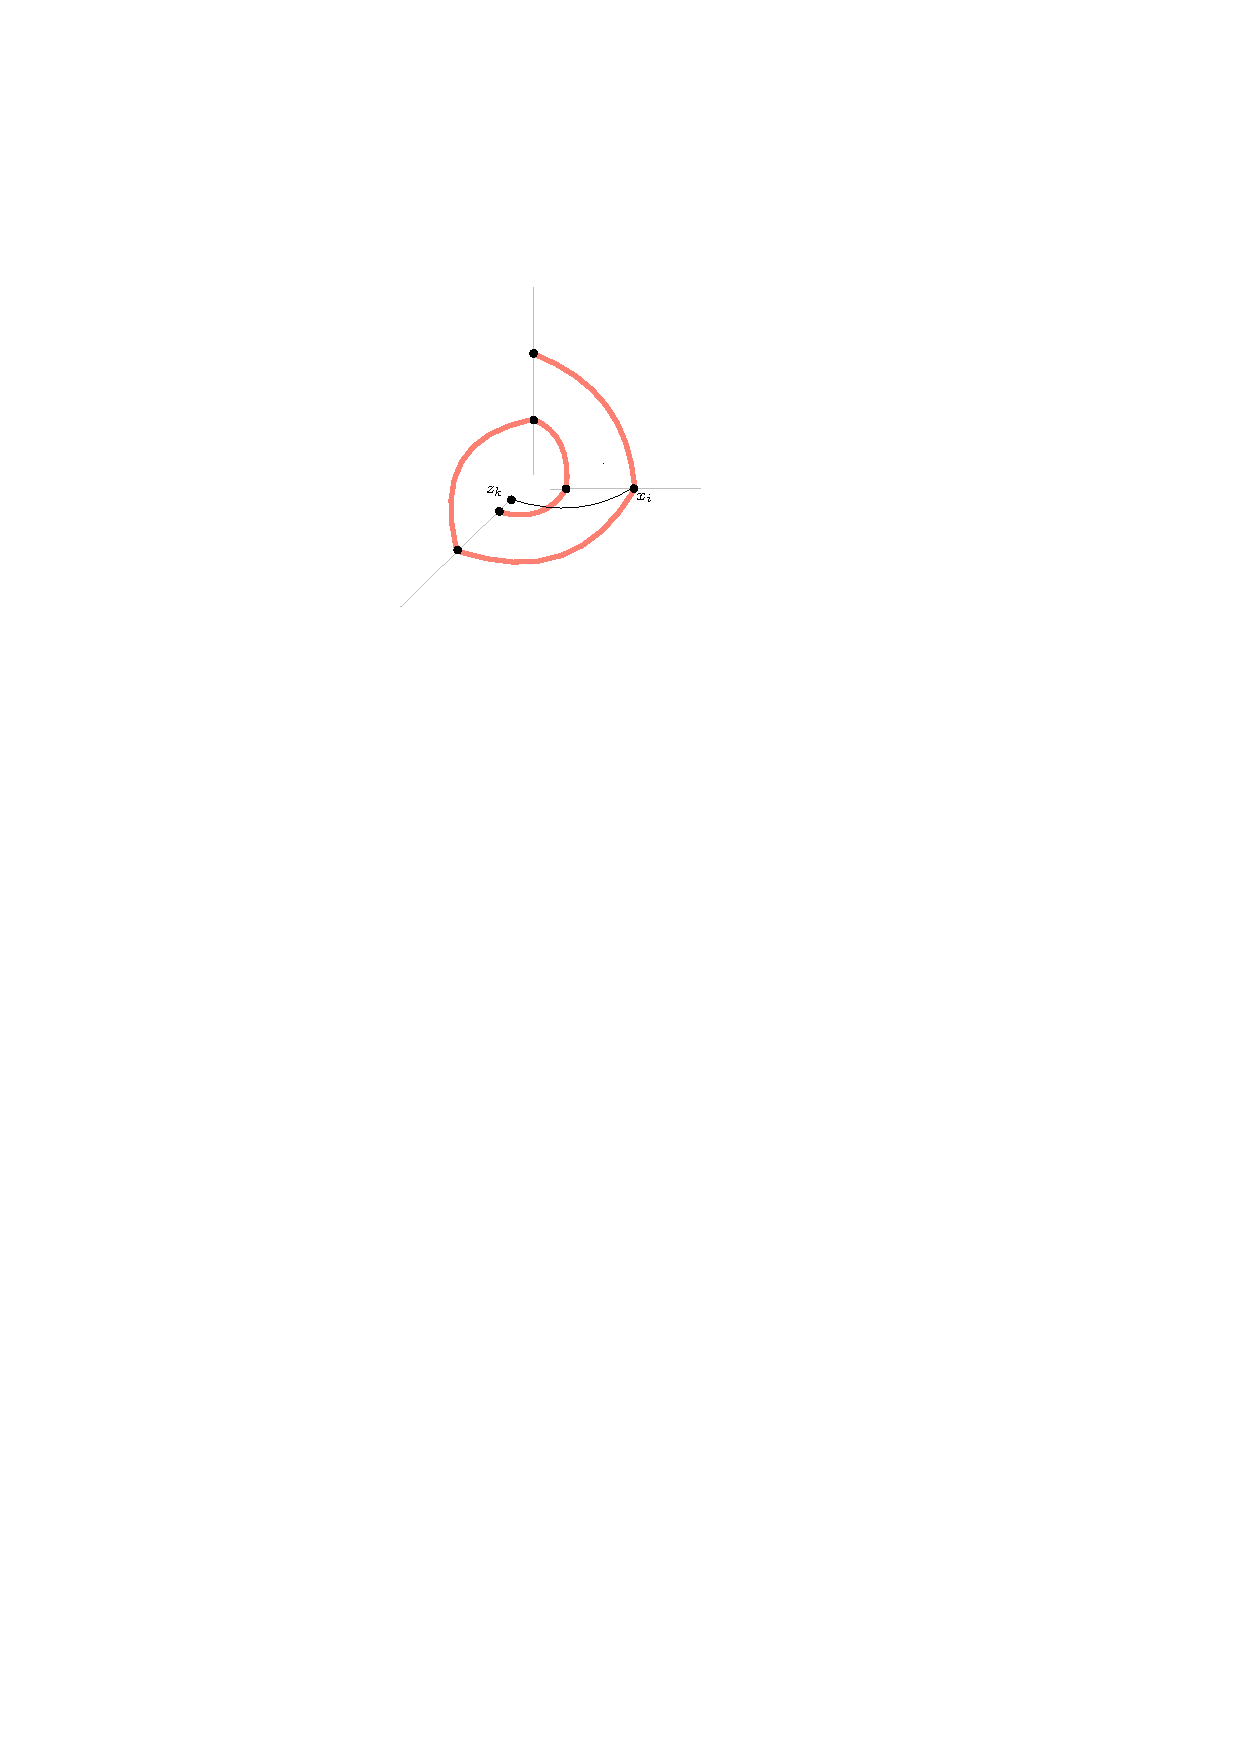
\includegraphics[width=40mm]{figs/2layermaximum-7} \caption{}\end{subfigure}
    \caption{The edge between a vertex $x_i$ and a vertex $y_j$ or $z_k$ cannot span more than 2 layers}
   \figlabel{2layermaximum}
 \end{center}
    \end{figure}

  \begin{enumerate}
  	\item$\ell(y_j) =  m+3n$ where $n \geq 1$. This edge cannot exist since it would contradict our greedy path constructing algorithm.
  	\item$\ell(y_j) =  m+1$. This edge will only span one layer.
  	\item $\ell(y_j) = m+1-3n$ where $n \geq 1$. This edge cannot exist, since it would create a crossing with the edge $v_{m-3}v_{m-2}$.
  \end{enumerate}

  Second, we look at the possible cases for an edge between $x_i$ with $\ell(x_i) = m$ and $z_k$ where $z_k \notin P$.
 \begin{enumerate}
  \setcounter{enumi}{3}
  	\item $\ell(z_k) = m+2+3n$ where $n \geq 1$. This edge cannot exist, since it would create a crossing with the edge $v_{m+2}v_{m+3}$.
  	\item$\ell(z_k) =  m+2$. This edge spans exactly two layers.
  	\item$\ell(z_k) =  m-1$. This edge will only span one layer.
  	\item $\ell(z_k) =  m-1-3n$ where $n \geq 1$. This edge cannot exist, since it would create a crossing with the edge $v_{m-4}v_{m-3}$.
  \end{enumerate}


  Next, we will need a notion of levelled planar graphs. The class of levelled
  planar graphs was introduced in 1992 by Heath and Rosenberg
  \cite{HR-SJC92} in their study of queue layouts of graphs. A \emph{levelled
  planar drawing} of a graph is a straight-line crossing-free drawing in
  the plane, such that the vertices are placed on a sequence of parallel
  lines (called levels), where each edge joins vertices in two
  consecutive levels. A graph is \emph{levelled planar} if it has a levelled
  planar drawing. (This is a well studied model for planar
  graph drawing, known as a Sugiyama-style drawing \cite{STT81,BM2001,HN2013,BETT99}.)

  Now, consider the graph $G-P$ obtained by removing the vertices of $P$
  from $G$ (see \figref{g-p}).  We claim that this graph is a levelled
  planar graph in which the levels
  of the vertices are given by the layering $\ell$ defined above. (Recall that the edges of $G$ spanning two layers all have at least one endpoint in $P$.)
  Refer to \figref{prism}. One way to see this is to imagine $G$
  as being drawn with its vertices on the three vertical edges of the surface of
  a triangular prism so that $x_1,y_1,z_1$ are the vertices of one
  triangular face and $x_{n_1},y_{n_2},z_{n_3}$ are the vertices of
  the other triangular face.  Now, if we remove the triangular faces
  of this prism, cut it along the embedding of $P$, and unfold
  the resulting surface so that it lies in the plane, then we obtain a
  drawing of $G-P$ in which the vertices lie on a set of parallel lines
  and in which the edges only join vertices on two consecutive lines.
  This gives the desired levelled planar drawing of $G-P$.

  % See \figref{g-p} for an example of the constructed path $P$.

  \begin{figure}
  \begin{center}
  \begin{tabular}{cc}
  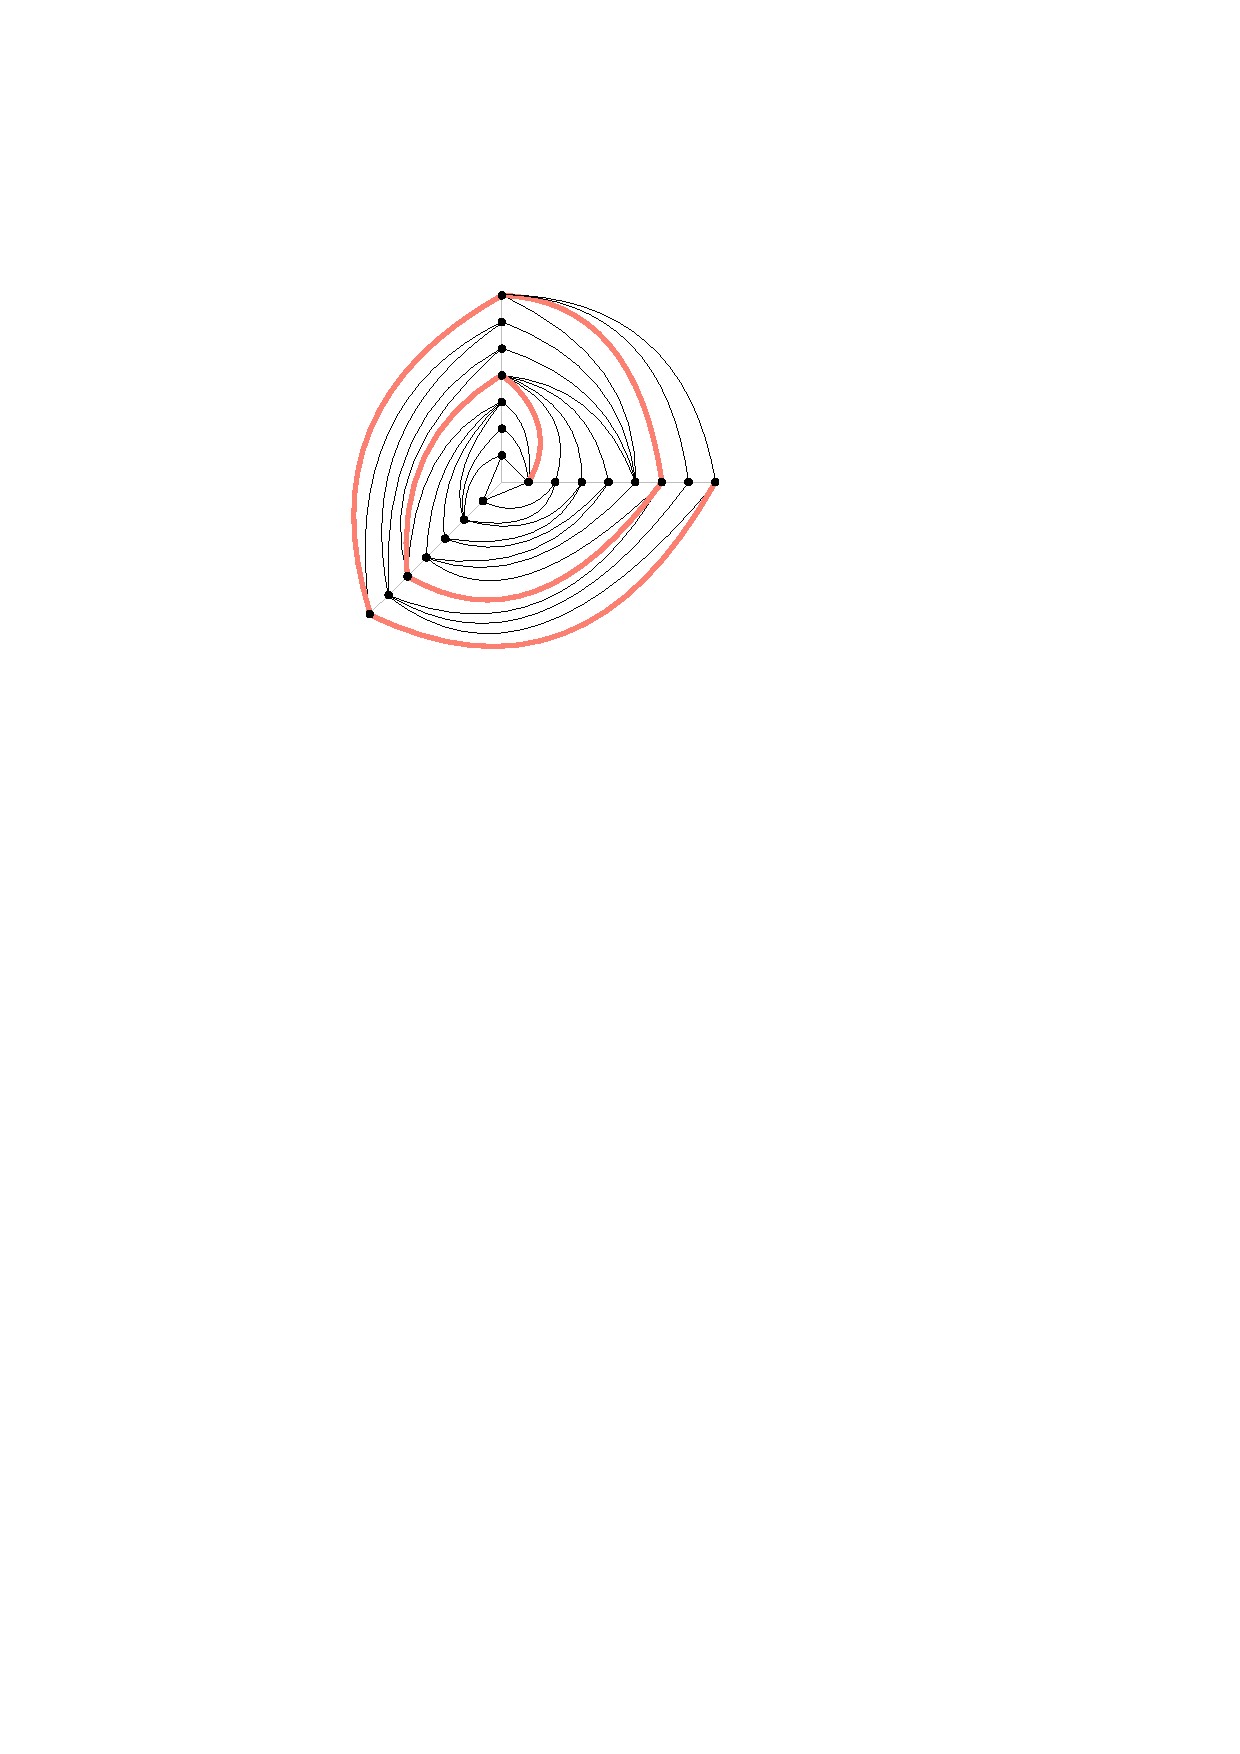
\includegraphics{figs/graph-2}
  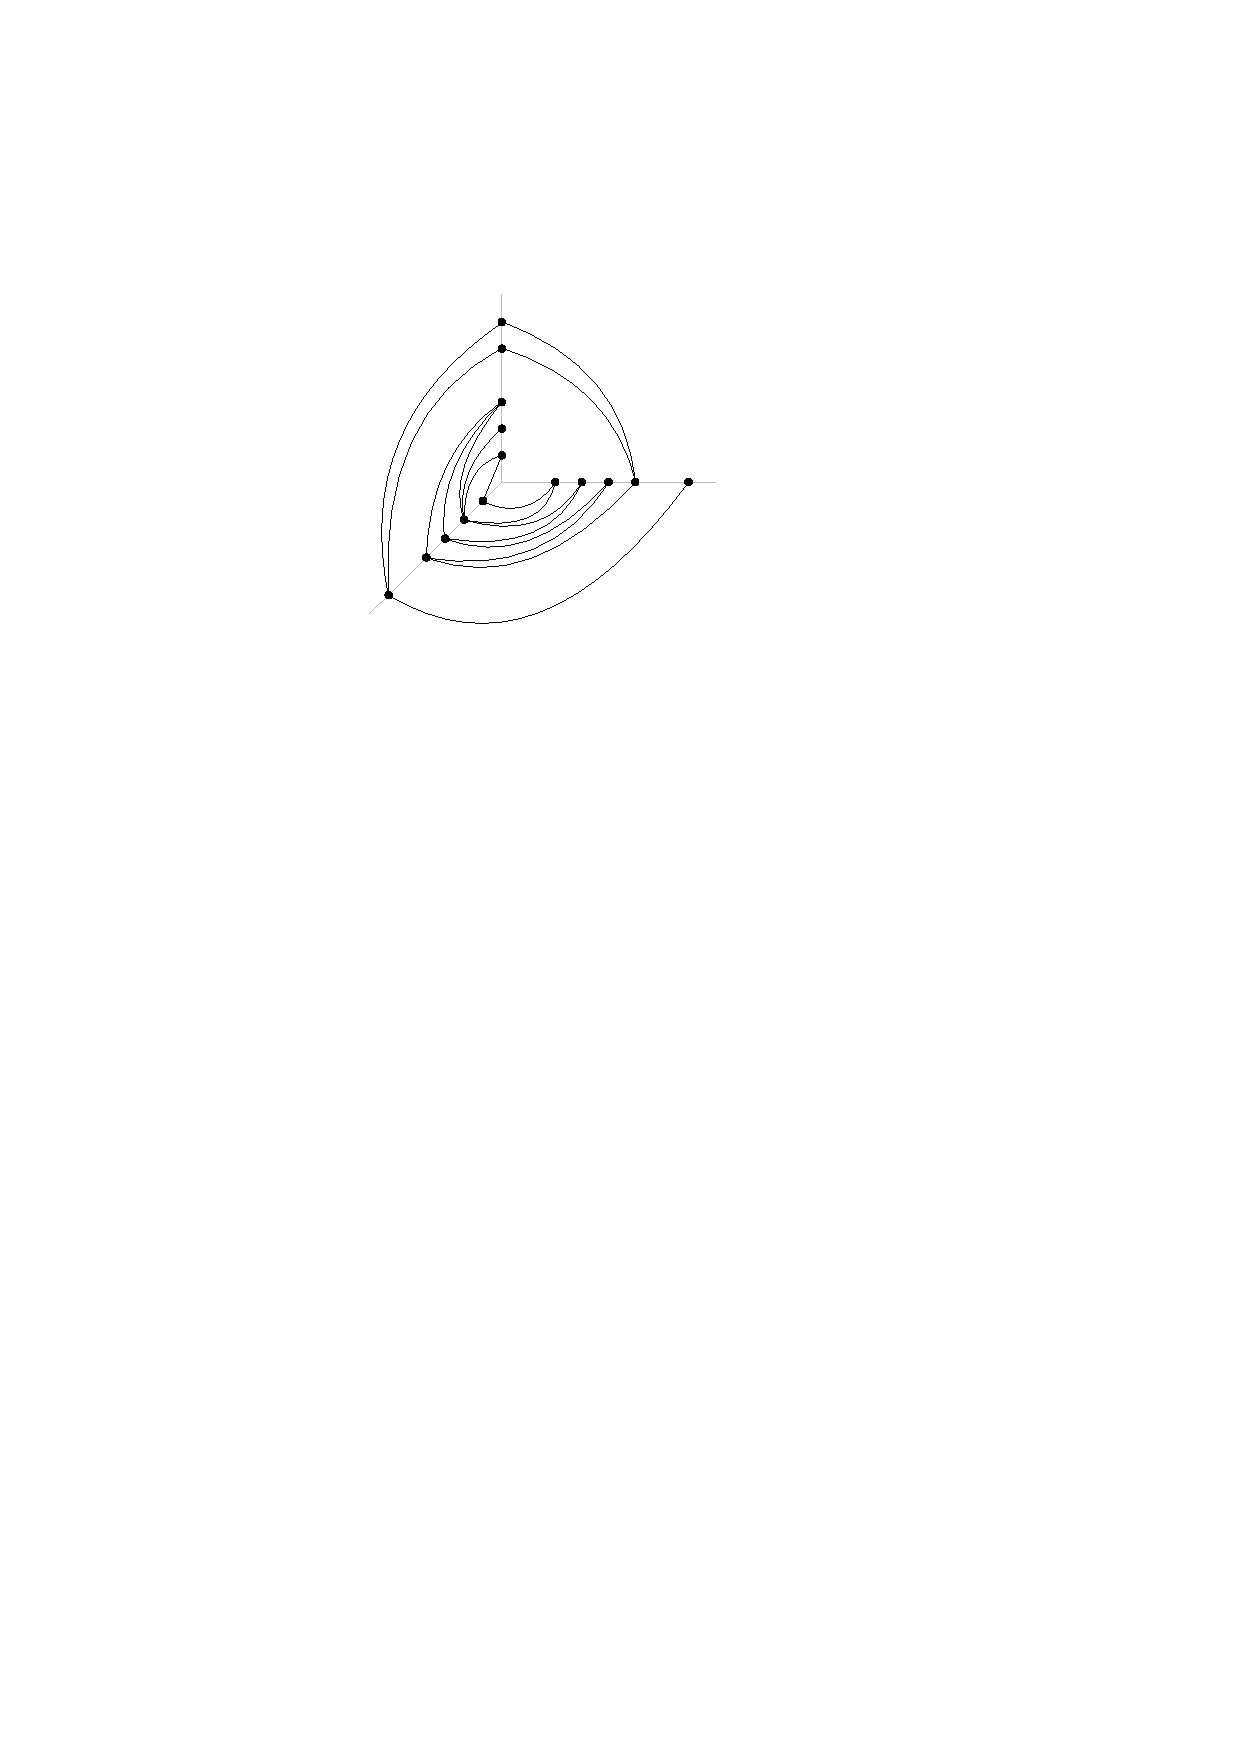
\includegraphics{figs/graph-3}
  \end{tabular}
  \end{center}
  \caption{The graph $G-P$ is a levelled planar graph.}
  \figlabel{g-p}
  \end{figure}

  \begin{figure}
   \begin{center}
      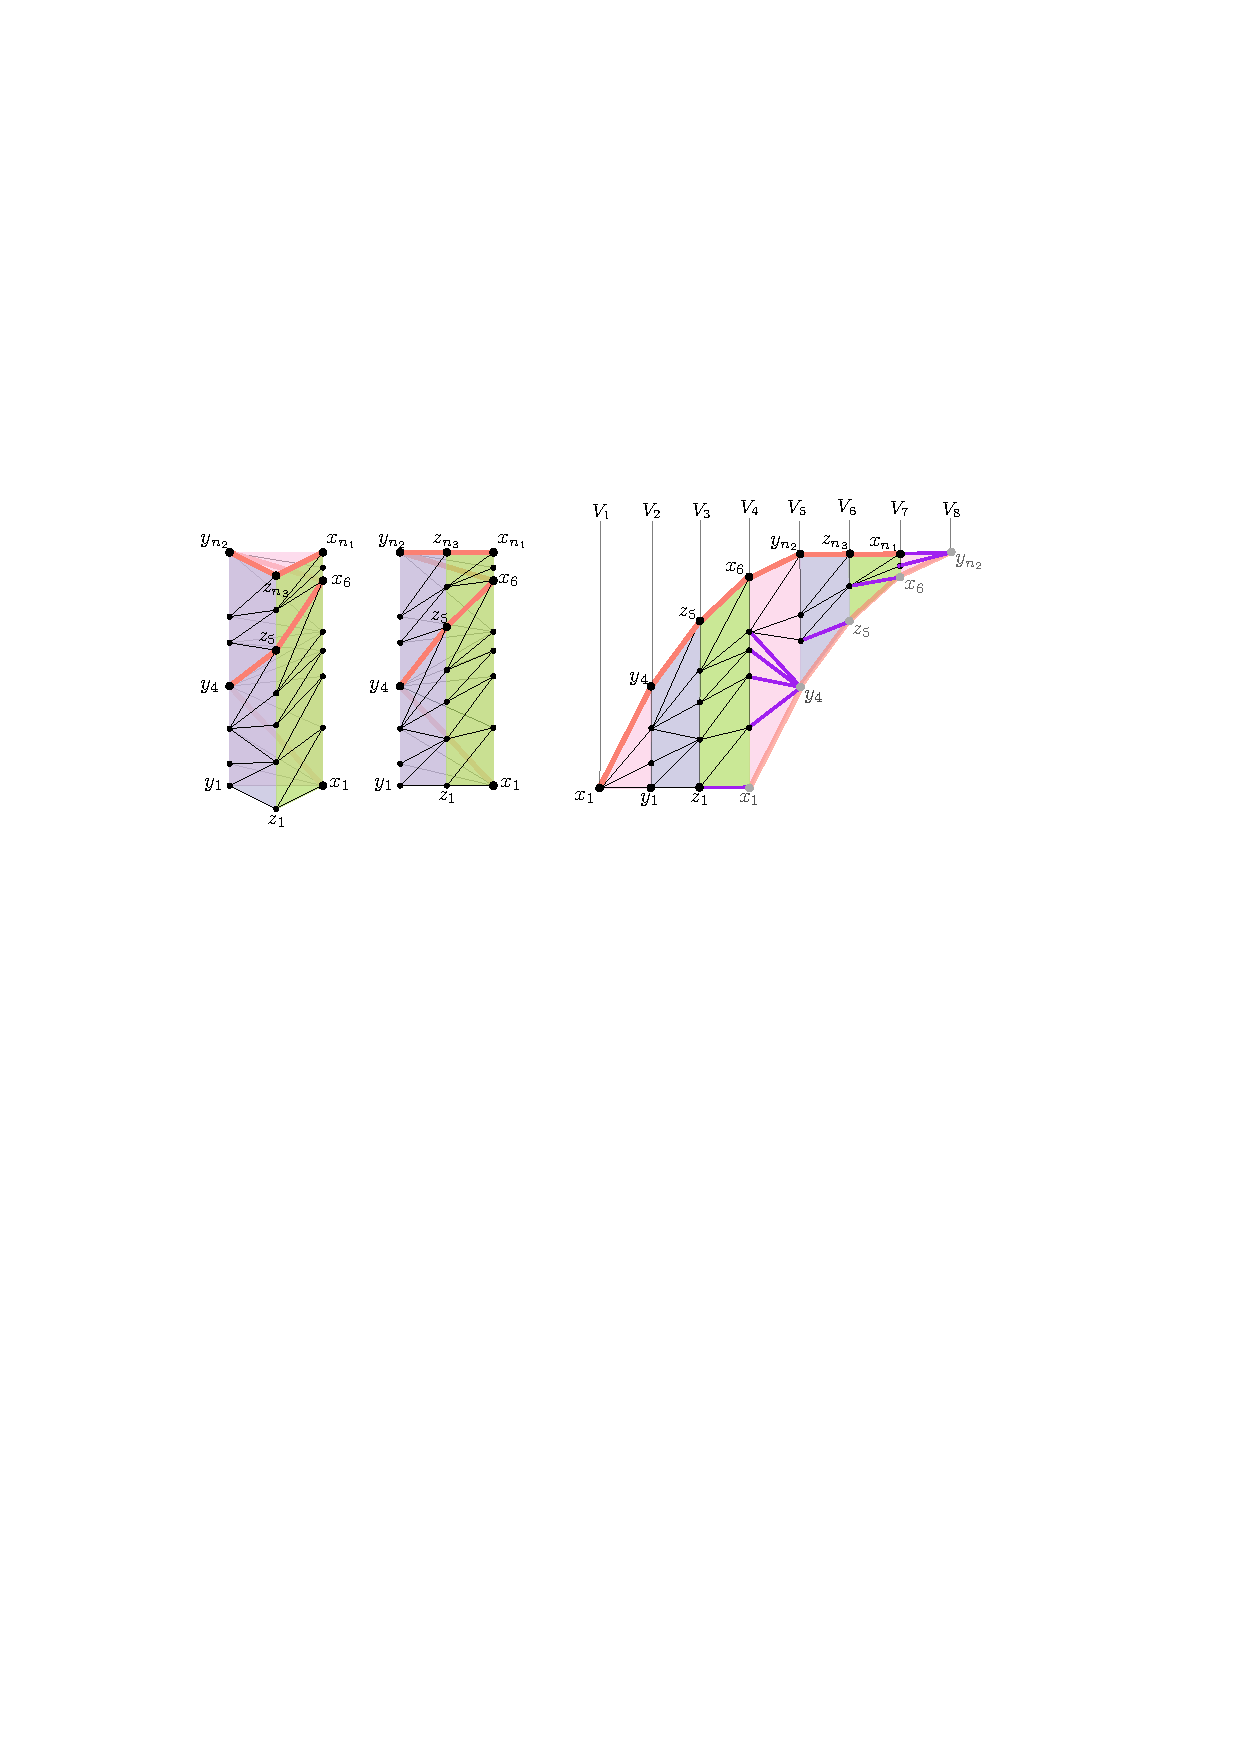
\includegraphics[width=0.95\columnwidth]{figs/prism}
   \end{center}
   \caption{Cutting a prism along $P$ to obtain a levelled planar
    drawing of $G-P$. Edges that span 2 layers are drawn in purple.}
   \figlabel{prism}
  \end{figure}

  \begin{figure}
   \begin{center}
      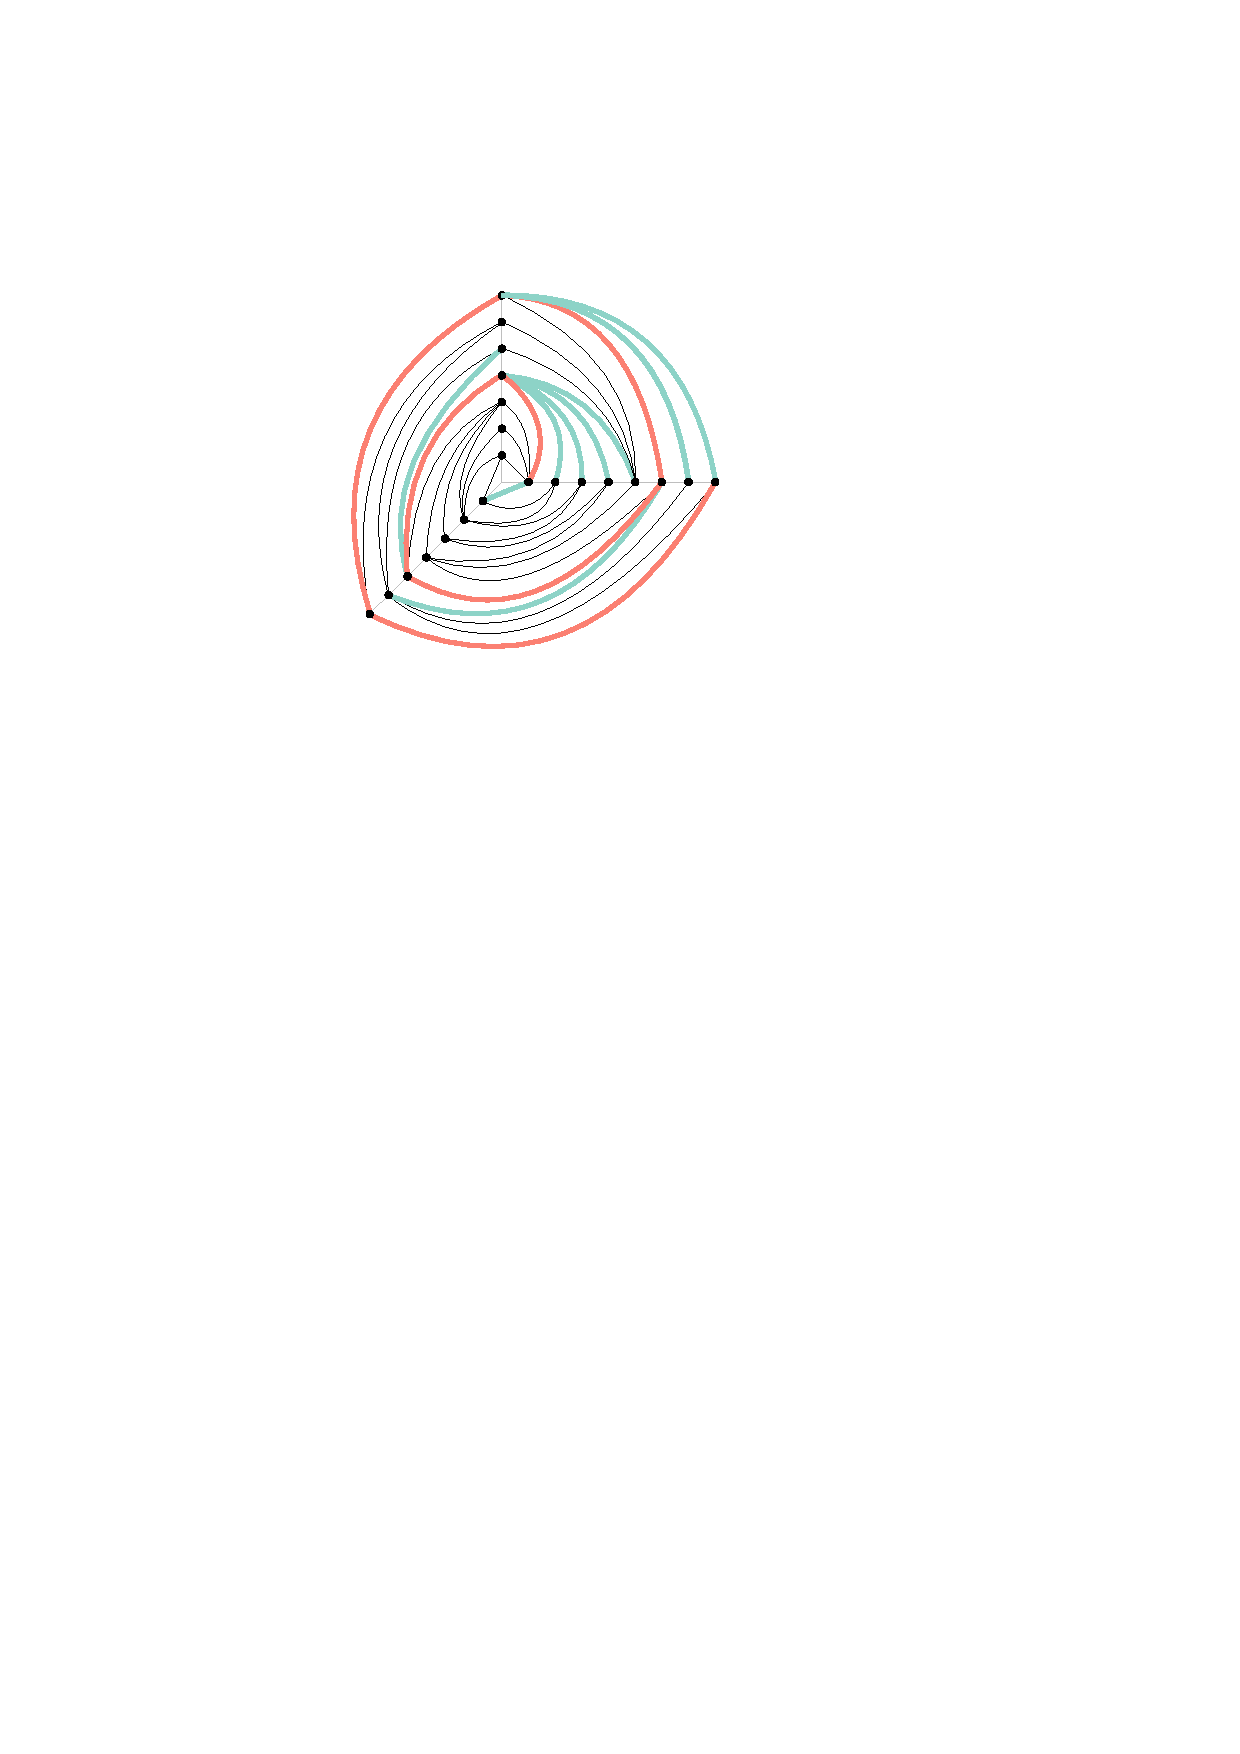
\includegraphics{figs/prism_graph-3}
   \end{center}
   \caption{The graph G with the path P and edges that span 2 layers drawn in purple}
   \figlabel{graph2layers}
  \end{figure}

  By a result of Bannister \etal\ \cite[Proof of
  Theorem~5]{bannister2018track}, $G-P$ has a layered
  path decomposition $B_1,\ldots,B_p$ of width 1 using the layering
  $\ell$ defined above.  If we add the vertices of $P$ to every bag
  of this decomposition we obtain a width-2 2-weak layered path
  decomposition of $G$.  Finally, to satisfy Conditions 2 and 4 of
  the lemma, we prepend a bag $B_0=\{x_1,y_1,z_1\}$ and append a bag
  $B_{p+1}=\{x_{n_1},y_{n_2},z_{n_3}\}$.
\end{proof}

%
%
%
%
%
%
% \begin{proof}[Sketch of proof of \lemref{main}]
% %
% % In this section, we will only present a brief sketch of the proof of \lemref{main}, and have provided the complete proof of  in \appref{appendix}.
%
%
%  % 1. The induction proof, the base case, and the induction step
%  The proof is by induction on the number $|V(G)|$ of vertices.
%   If $|V(G)|\le 4$, then the result is trivial.
%
%   Suppose that $G$ has
%   a cut set $C=\{x_i,y_j,z_k\}$ having exactly one vertex in each track.
%   Since $G$ is edge-maximal, $x_i,y_j,z_k$ form a cycle in $G$.  Now,
%   the subgraph $G_1$ of $G$ induced by $\{x_1,\ldots,x_i, y_1,\ldots,y_j,
%   z_1,\ldots,z_k\}$ is an edge-maximal graph with $\tr(G_1)=3$.
%   Similarly, the subgraph $G_2$ of $G$ induced by $\{x_i,\ldots,x_{n_1},y_j,\ldots,y_{n_2},z_k,\ldots,z_{n_3}\}$ is edge-maximal with $\tr(G_2)=3$.  We can therefore apply the lemma inductively on each of $G_1$ and $G_2$. By appropriately relabelling $x$, $y$, and $z$ in $G_2$, Conditions~2 and 4 of the lemma ensure that the desired path decomposition of $G$ can be obtained by concatenating the path decompositions of $G_1$ and $G_2$.  Conditions~3 and 5 ensure that a layering of $G$ can be obtained by combining the layering of $G_1$ with (a shifted version) the layering of $G_2$.
%   %
%   %
%   %
%   %  and we
%   % can inductively apply \lemref{main} to find a 2-weak layered
%   % path decomposition of width 2 for $G_1$ in which $x_i,y_j,z_k$ are in the last bag
%   % and are assigned to three consecutive distinct layers $r+1$, $r+2$, and $r+3$.
%   % Note that there are three possible assignments of $x_i,y_j,z_k$ to
%   % these three layers depending on the value of $r\bmod 3$.
%   % For the subgraph $G_2$ induced by $\{x_i,\ldots,x_{n_1},y_j,\ldots,y_{n_2},z_k,\ldots,z_{n_3}\}$,
%   % we apply \lemref{main} inductively, relabelling tracks to
%   % ensure that in the resulting layered decomposition $\ell(y_j)=1$,
%   % $\ell(z_k)=2$ and $\ell(x_i)=3$.   We can now obtain a width-2 2-weak
%   % layered path decomposition of $G$ by joining the two decompositions.
%   % In particular, concatenating the sequence of bags for $G_1$ with
%   % the sequence of bags for $G_2$ gives a path decomposition of $G$
%   % and adding $r$ to the indices of all layers in the layering of $G_2$
%   % gives a 2-weak layering of $G$.
%
%
%  % 2. The furthest vertex path P
%  Thus, we can focus on case where $G$ has no separating triangle. In this case, we greedily construct a path $P= v_1, ..., v_r$. The first vertex of $P$ will be one
%  of $x_1, y_1, z_1$ and the last three vertices will be $x_{n_1}, y_{n_2}, z_{n_3}$.
%  For any $v_k \in P$, we select the next vertex $v_{k+1}$ by
% choosing the neighbouring vertex of $v_k$ on track $T_{k+1}$ with the highest index.
% See \figref{g-p} for an example of the constructed path $P$.
%
% \begin{figure}[H]
% \begin{center}
% \begin{tabular}{cc}
% 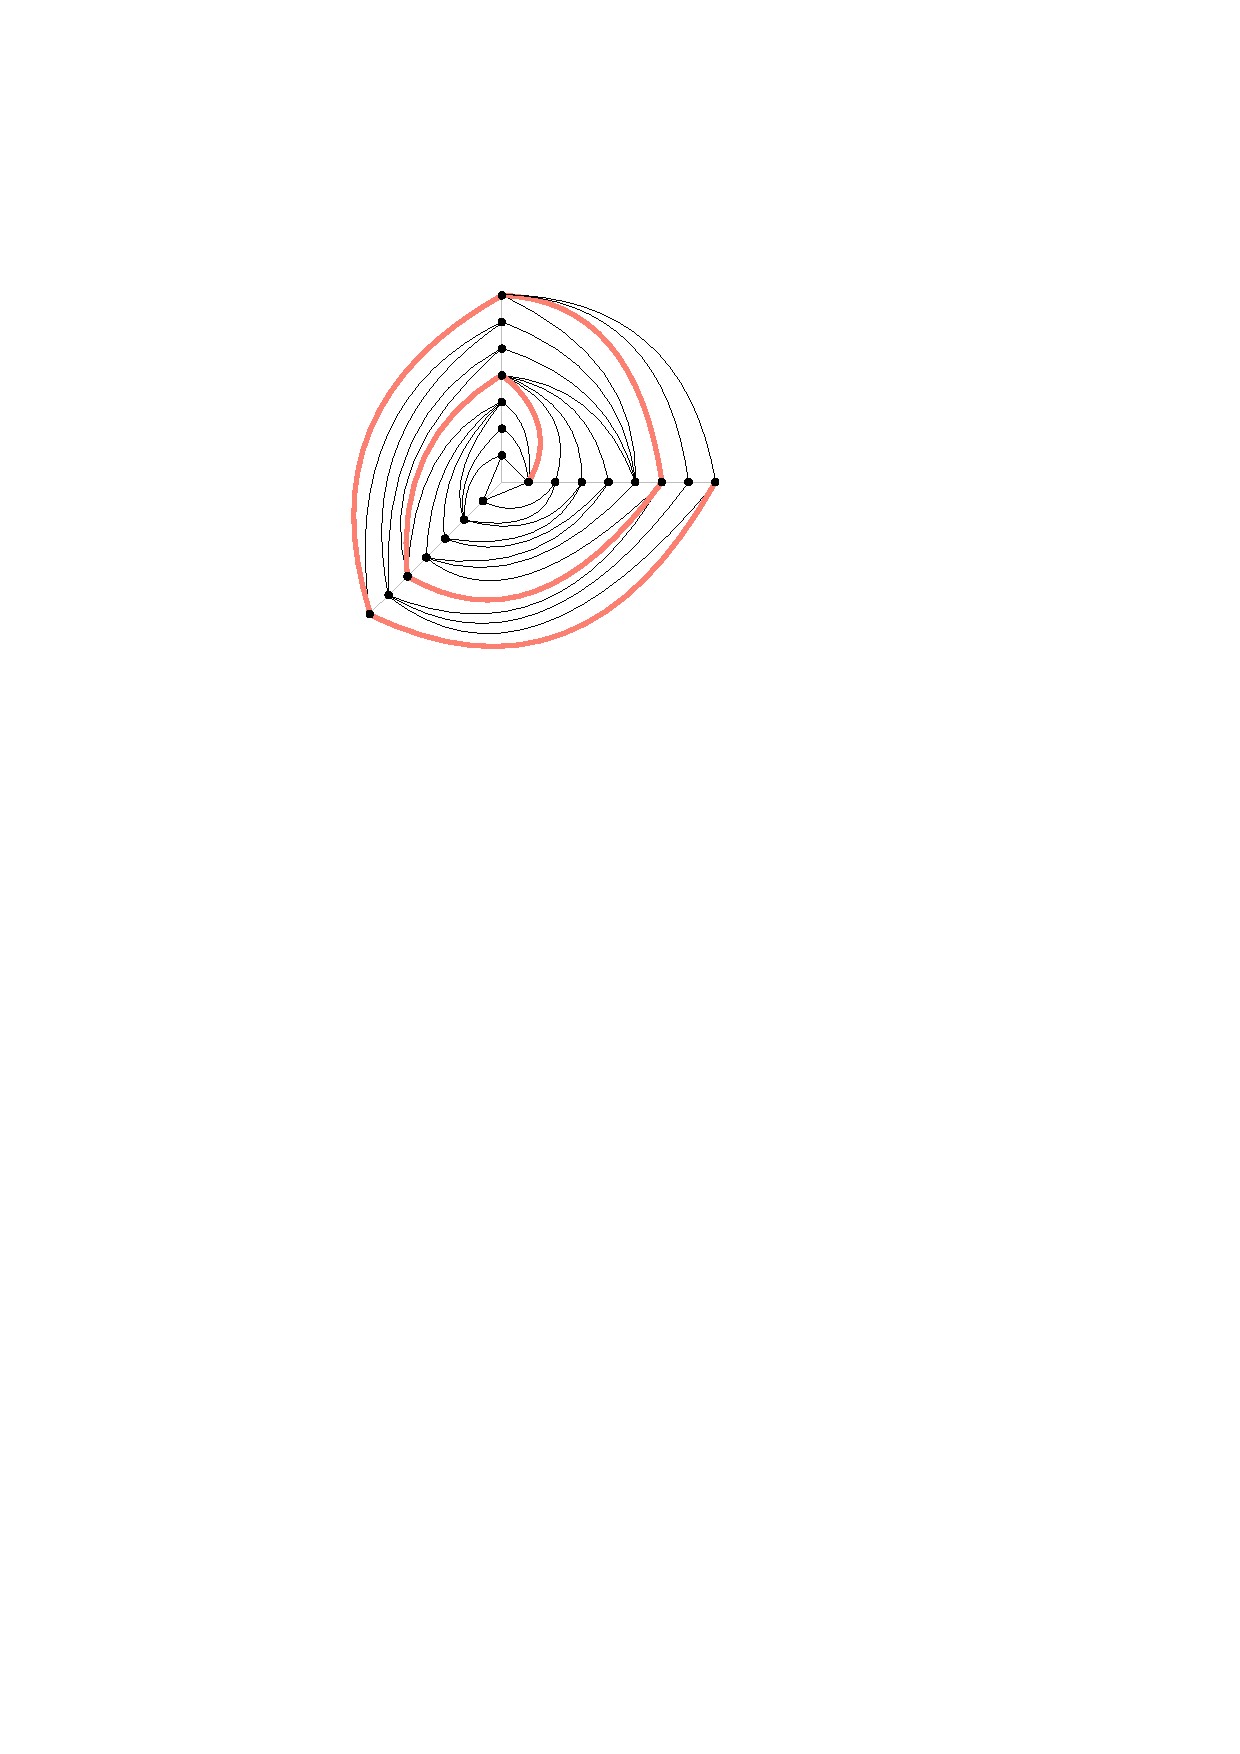
\includegraphics{figs/graph-2}
% 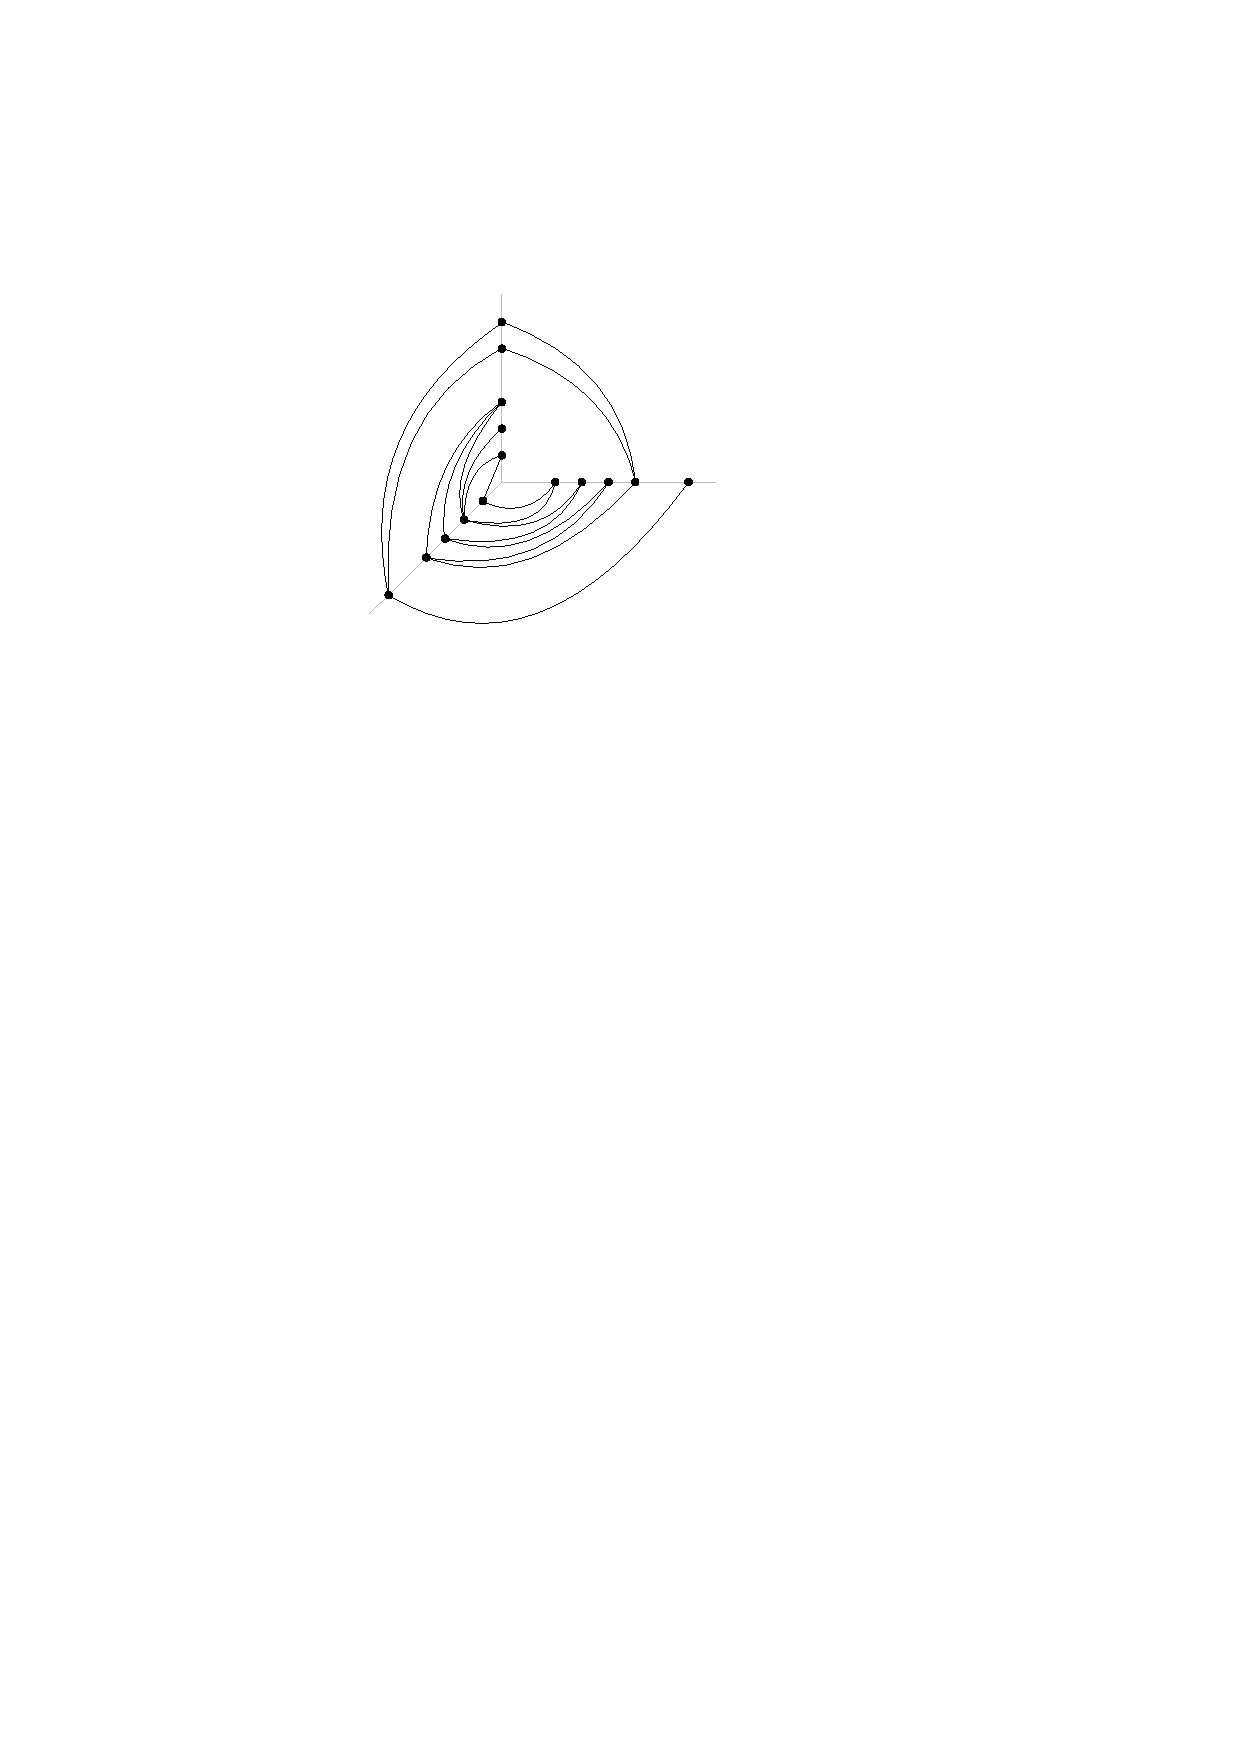
\includegraphics{figs/graph-3}
% \end{tabular}
% \end{center}
% \caption{The graph $G-P$ is a levelled planar graph.}
% \figlabel{g-p}
% \end{figure}
%
%
% % 3.  2-weak-layering
% The 2-weak layering of $G$ is obtained as follows: For each vertex $v_i$ on $P$, we will set $\ell(v_i) = i$
% For each $t\in\{1,2,3\}$, any vertex $v\in T_t$ that is not in $P$ is assigned to the same layer as $v$'s immediate successor in $P\cap T_t$.  That this is a 2-weak layering follows from straightforward analysis. (The only edges that span 2 layers are those incident to a vertex in $v\in T_{i-1}\setminus V(P)$ and a vertex $v_i\in T_{i}\cap V(P)$, where $v$ is further from the origin than $v_{i-1}$.)
% %
% %
% %
% % Careful 2-weak layering of $G$. The proof for this is provided in the Appendix.
%
% % 4.  G-P is levelled planar
% % Next, we will need a notion of levelled planar graphs. The class of levelled
% % planar graphs was introduced in 1992 by Heath and Rosenberg
% % \cite{HR-SJC92} in their study of queue layouts of graphs. A levelled
% % planar drawing of a graph is a straight-line crossing-free drawing in
% % the plane, such that the vertices are placed on a sequence of parallel
% % lines (called levels), where each edge joins vertices in two
% % consecutive levels. A graph is levelled planar if it has a levelled
% % planar drawing. (This is a well studied model for planar
% % graph drawing, so called Sugiyama-style \cite{STT81,BM2001,HN2013,BETT99}.)
% % Now, consider the graph $G-P$ obtained by removing the vertices of $P$
% % from $G$ (see \figref{g-p}).  We claim that this graph is a levelled
% % planar graph in which the levels of the vertices are given by the layering $\ell$ defined above.
%
% Next, we consider the graph $G-P$ obtained by removing the vertices of $P$ from $G$.  Clearly $\tr(G-P)\le 3$ and, since every edge of $G-P$ joins a pair of vertices in two consecutive layers, every cycle in $G-P$ has even length, so $G-P$ is bipartite.
% By a result of Bannister \etal\ \cite[Proof of Theorem~5]{bannister2018track}, $G-P$ has a layered
% path decomposition $B_1,\ldots,B_p$ of width 1 using the layering
% $\ell$ defined above.  If we add the vertices of $P$ to every bag
% of this decomposition we obtain a width-2 2-weak layered path
% decomposition of $G$.  Finally, to satisfy Conditions 2 and 4 of
% the lemma, we prepend a bag $B_0=\{x_1,y_1,z_1\}$ and append a bag
% $B_{p+1}=\{x_{n_1},y_{n_2},z_{n_3}\}$.
% \end{proof}


% Bibliography
\bibliographystyle{plain}
\bibliography{lpw}

\end{document}
